\documentclass[../main.tex]{subfiles}
\usepackage{tikz}
\usetikzlibrary{arrows.meta,positioning,shapes.geometric}
\begin{document}

\section{Tổng quan phương pháp nghiên cứu}
\label{sec:methodology-overview}

Chương này trình bày phương pháp thực nghiệm của đồ án: xây dựng môi trường mô phỏng hệ thống điều khiển công nghiệp, tái hiện các hành vi tấn công điển hình trên giao thức S7comm, phân tích lưu lượng mạng thu được, tạo cơ sở phục vụ xây dựng luật phát hiện bằng IDS Suricata ở các chương tiếp theo.

Quy trình nghiên cứu được tổ chức thành năm bước liên tiếp như sau.

\begin{enumerate}
    \item \textbf{Thiết lập môi trường thí nghiệm}: triển khai môi trường mô phỏng trên phần mềm ảo hoá VMWare sử dụng các máy ảo:
    \begin{itemize}
        \item PLC mô phỏng thông qua OpenPLC Runtime v4
        \item HMI thông qua FUXA
        \item Ubuntu Desktop/Server cho máy của kẻ tấn công, Router và IDS.
    \end{itemize}

    \textit{Ngoài ra trong một số kịch bản có sử dụng phần mềm TIA Portal + S7-PLCSIM Advanced + WinCC để mô phỏng PLC và HMI do giới hạn mô phỏng của OpenPLC Runtime v4.}
  
    \item \textbf{Mô phỏng kịch bản tấn công}: thực hiện trinh sát, phát lại lệnh Start/Stop, thao tác upload/download, DoS và gói tin malformed trên kênh S7comm, cùng tấn công man-in-the-middle trên giao thức S7comm.
    
    \item \textbf{Thu thập và phân tích lưu lượng}: thu thập lưu lượng mạng bằng Wireshark, phân tích cấu trúc gói tin S7comm để tạo cơ sở phục vụ xây dựng luật phát hiện bằng IDS Suricata.
    
    \item \textbf{Xây dựng luật phát hiện}: chuyển các dấu hiệu đã quan sát thành chữ ký Suricata (\texttt{s7comm.rules}, \texttt{ics\_dos.rules}, \texttt{s7comm\_malformed.rules}), căn cứ offset byte, mã chức năng, ngưỡng tần suất (DoS) và cú pháp bất thường (malformed).
    
    \item \textbf{Kiểm thử IDS}: chạy Suricata trên bản sao lưu lượng, đối chiếu cảnh báo với từng kịch bản đã mô phỏng.
    
\end{enumerate}

Hình~\ref{fig:methodology-flow} mô tả luồng hoạt động tổng thể của giải pháp đề xuất. 

\begin{figure}[H]
    \centering
    \begin{tikzpicture}[
        node distance=0.55cm and 0.35cm,
        box/.style={draw, rounded corners, align=center, font=\small,
            minimum width=2.35cm, minimum height=0.85cm},
        arr/.style={-{Stealth[length=2mm]}, thick}
    ]
        \node[box] (lab) {Thiết lập\\môi trường lab};
        \node[box, right=of lab] (atk) {Mô phỏng\\kịch bản tấn công};
        \node[box, right=of atk] (pcap) {Thu thập\\PCAP};
        \node[box, right=of pcap] (ana) {Phân tích\\S7comm};
        \node[box, right=of ana] (ids) {Luật Suricata\\và kiểm thử};
        \draw[arr] (lab) -- (atk);
        \draw[arr] (atk) -- (pcap);
        \draw[arr] (pcap) -- (ana);
        \draw[arr] (ana) -- (ids);
    \end{tikzpicture}
    \caption{Luồng phương pháp nghiên cứu của đồ án}
    \label{fig:methodology-flow}
\end{figure}

Phạm vi chương này dừng ở bước phân tích lưu lượng và mô tả kịch bản; việc viết luật Suricata và đánh giá độ chính xác cảnh báo được trình bày ở chương sau.

\section{Thiết lập môi trường thí nghiệm}
\label{sec:lab-setup}

\subsection{Nguyên tắc triển khai}

Môi trường lab được thiết kế theo hướng mô phỏng có kiểm soát trên máy ảo. Tất cả các máy ảo được triển khai sử dụng đối tượng LAN Segment của VMWare (sử dụng 2 LAN Segment: 192.168.50.0/24 cho Controller Layer và 192.168.60.0/24 cho Superuser Layer). Hệ thống IDS được triển khai ở dạng Passive mode bằng cách đặt trong cùng LAN Segment. 

Do cách hoạt động đặc biệt của VSwitch trong VMWare giống với hub thông thường thay vì switch nên chỉ cần IDS đặt trong cùng LAN Segment và bật chế độ Promiscuous mode cho card mạng là có tác dụng tương đương SPAN/mirror port trên một switch được triển khai vật lý. Hình~\ref{fig:lab-topology} mô tả cách hai LAN Segment được nối và các máy chủ mang lưu lượng S7comm trong cấu hình lab mặc định.

\begin{figure}[htbp]
    \centering
    
\includegraphics[width=0.95\textwidth]{Figure/lab_topology.png}
    \caption{Sơ đồ topology lab trên VMware LAN Segment. \textbf{Controller Layer} (\texttt{192.168.50.0/24}): OpenPLC RUNTIME tại \texttt{192.168.50.10}. \textbf{Superuser Layer} (\texttt{192.168.60.0/24}): FUXA EDITOR tại \texttt{192.168.60.10}. Router ảo (\texttt{192.168.50.1}/\texttt{192.168.60.1}) định tuyến giữa hai segment. Mũi tên đen: yêu cầu/phản hồi Read Var của HMI; mũi tên đỏ: Write Var của kẻ tấn công và phản hồi Read Var bị sửa (kịch bản MITM, Mục~\ref{sec:stuxnet_mitm_sim}). Máy IDS (\texttt{172.16.16.7}) cùng segment Controller ở chế độ promiscuous, không vẽ trên sơ đồ cho gọn.}
    \label{fig:lab-topology}
\end{figure}

\subsection{Công cụ sử dụng}

\textbf{OpenPLC} là một nền tảng mã nguồn mở cho phép  mô phỏng một PLC vật lý trên máy tính. Phần mềm tương thích với Windows, Linux, macOS, Raspberry Pi. Nó hỗ trợ chương trình điều khiển theo chuẩn IEC 61131-3, cho phép kết nối với SCADA, HMI, hoặc thiết bị công nghiệp khác. OpenPLC có 2 phần chính:

- \href{https://autonomylogic.com/runtime}{\textbf{OpenPLC Runtime}}: đây là PLC engine giúp mô phỏng một PLC vật lý. OpenPLC Runtime V4 hỗ trợ nhiều giao thức công nghiệp, trong đó có giao thức Siemens S7comm. Khi kích hoạt giao thức này trên OpenPLC Runtime V4, runtime sẽ lắng nghe cổng 102 và phục vụ giao thức Siemens S7comm thông qua driver Snap7 bên trong. Đồ án sử dụng OpenPLC Runtime V4.

Hình~\ref{fig:S7_on_OpenPLC} minh họa S7comm được kích hoạt trên OpenPLC Runtime V4.

\begin{figure}[H]
    \centering
    
\includegraphics[width=0.9\textwidth]{Figure/S7_on_OpenPLC.png}
    \caption{S7comm được kích hoạt trên OpenPLC Runtime V4}
    \label{fig:S7_on_OpenPLC}
\end{figure}


- \href{https://autonomylogic.com/download}{\textbf{OpenPLC Editor}}: Đây là IDE để viết chương trình dành cho OpenPLC Runtime. Nó tương tác với OpenPLC Runtime thông qua Restful API cổng 8443. Trong đồ án sử dụng để viết code, complie chương trình, nạp chương trình vào PLC và debug chương trình. Đồ án sử dụng OpenPLC Editor V4.

Hình~\ref{fig:OpenPLC_Editor} minh họa openPLC Editor để viết chương trình, biên dịch chương trình, nạp vào runtime và debug.

\begin{figure}[H]
    \centering
    
\includegraphics[width=0.9\textwidth]{Figure/OpenPLC_Editor.png}
    \caption{OpenPLC Editor để viết chương trình, biên dịch chương trình, nạp vào runtime và debug}
    \label{fig:OpenPLC_Editor}
\end{figure}

\textbf{FUXA} (Docker \texttt{frangoteam/fuxa:snap7}, cổng 1881) đóng vai trò thiết kế và hiển thị giao diện HMI. Đây là một HMI mã nguồn mở, có hỗ trợ giao thức Siemens S7comm và chạy trên nền web.

Hình~\ref{fig:FUXA} minh họa fUXA để thiết kế và hiển thị giao diện HMI.

\begin{figure}[H]
    \centering
    \includegraphics[width=0.9\textwidth]{Figure/FUXA.png}
    \caption{FUXA để thiết kế và hiển thị giao diện HMI}
    \label{fig:FUXA}
\end{figure}


\textbf{Snap7}: một thư viện mã nguồn mở được phát triển để kết nối, truyền và điều khiển các thiết bị tự động hóa, là một trong những thư viện mã nguồn mở phổ biến nhất trong ngành tự động hóa.

Snap7 hỗ trợ các giao thức truyền thông Siemens S7 (S7comm) để kết nối và truyền dữ liệu với các thiết bị tự động hóa Siemens. Nó cung cấp các tính năng chính như:

\begin{itemize}
    \item Đọc và ghi các biến trong PLC
    \item Truy cập vào các khối DB và OB trong PLC
    \item Cung cấp các thông tin về trạng thái của thiết bị
\end{itemize}

Các đặc điểm của Snap7: 

\begin{itemize}
    \item Có thể được sử dụng với nhiều ngôn ngữ lập trình phổ biến như C++, C#, Python, Java cho phép lập trình viên lựa chọn ngôn ngữ phù hợp nhất với dự án của mình. 
    \item Hoạt động trên nhiều hệ điều hành, bao gồm Windows, Linux, và macOS, mang lại sự linh hoạt cao trong việc phát triển ứng dụng.
    \item Tương thích với nhiều dòng PLC S7, hỗ trợ giao tiếp với các dòng PLC S7-200, S7-300, S7-400, S7-1200, và S7-1500, giúp dễ dàng tích hợp vào các hệ thống hiện có.
\end{itemize}

\subsection{Công cụ giao diện lab}
\label{sec:lab-gui}

Chạy thí nghiệm lặp lại bằng tay---SSH vào máy Attacker để chạy script, rồi SSH vào máy IDS để đọc log Suricata---vừa chậm vừa dễ sai. Hai ứng dụng desktop được bổ sung như một lớp điều khiển mỏng trên lab: chúng không triển khai logic tấn công mới, mà cung cấp một cửa sổ để kích hoạt các kịch bản đã mô tả ở các mục sau và quan sát phản hồi của cảm biến theo thời gian thực.

\textbf{Attack Tool.} Giao diện phía client dùng làm bảng điều khiển tạo lưu lượng S7comm. Người vận hành cấu hình PLC đích (địa chỉ, rack, slot) và máy Attacker từ xa, chọn loại kịch bản---trinh sát, ghi process, từ chối dịch vụ, gói malformed, hoặc phát lại Start/Stop---rồi bấm một lần để thực thi. Công cụ chạy script tương ứng trên Attacker qua SSH và hiển thị output trực tiếp trên panel log.

Hình~\ref{fig:demo-attack-recon} minh họa attack Tool: chọn kịch bản, cấu hình PLC/Attacker và log thực thi trực tiếp.

\begin{figure}[htbp]
    \centering
    
\includegraphics[width=0.82\textwidth]{Figure/Demo1.png}
    \caption{Attack Tool: chọn kịch bản, cấu hình PLC/Attacker và log thực thi trực tiếp.}
    \label{fig:demo-attack-recon}
\end{figure}

\textbf{Suricata Rules Tool.} Giao diện đồng hành kết nối tới máy IDS, hỗ trợ duyệt/sửa bộ luật S7comm, triển khai luật đã kiểm tra lên Suricata và theo dõi cảnh báo mới trên log cảm biến. Phạm vi mạng (\texttt{HOME\_NET}, interface bắt gói) có thể chỉnh trong cùng cửa sổ để khớp topology lab ở Hình~\ref{fig:lab-topology}.

Hình~\ref{fig:demo-rules-editor} minh họa suricata Rules Tool: danh sách luật, metadata và nội dung chữ ký có thể chỉnh sửa.

\begin{figure}[htbp]
    \centering
    
\includegraphics[width=0.82\textwidth]{Figure/Demo2.png}
    \caption{Suricata Rules Tool: danh sách luật, metadata và nội dung chữ ký có thể chỉnh sửa.}
    \label{fig:demo-rules-editor}
\end{figure}

Hình~\ref{fig:demo-rules-alerts} minh họa suricata Rules Tool: luồng cảnh báo trực tiếp khi lưu lượng tấn công được mirror tới IDS.

\begin{figure}[htbp]
    \centering
    
\includegraphics[width=0.82\textwidth]{Figure/Demo3.png}
    \caption{Suricata Rules Tool: luồng cảnh báo trực tiếp khi lưu lượng tấn công được mirror tới IDS.}
    \label{fig:demo-rules-alerts}
\end{figure}


\section{Kịch bản tấn công và phân tích lưu lượng}
\label{sec:attack-scenarios}

Phần dưới đây trình bày chi tiết các kịch bản đã mô phỏng. 

\subsection{Reconnaissance}
\label{sec:reconnaissance}

Sử dụng Nmap để quét thông qua NSE Scripts để phát hiện các thiết bị trong dải mạng. Script này sử dụng kỹ thuật quét riêng biệt dựa trên giao thức S7comm để tránh làm quá tải các thiết bị trong mạng OT.

\begin{verbatim}
nmap -p 102 --script s7-info <IP_ADDRESS>
\end{verbatim}

Output:

\begin{verbatim}
ubuntu@ubuntuserver2204:~$ nmap -p 102 --script s7-info 192.168.50.0/24
Starting Nmap 7.80 ( https://nmap.org ) at 2026-04-21 16:23 UTC
Nmap scan report for 192.168.50.1
Host is up (0.0018s latency).

PORT    STATE  SERVICE
102/tcp closed iso-tsap

Nmap scan report for 192.168.50.10
Host is up (0.0027s latency).

PORT    STATE SERVICE
102/tcp open  iso-tsap
| s7-info:
|   Module: 6ES7 315-2EH14-0AB0
|   Basic Hardware: 6ES7 315-2EH14-0AB0
|   Version: 3.2.6
|   System Name: SNAP7-SERVER
|   Module Type: CPU 315-2 PN/DP
|   Serial Number: S C-C2UR28922012
|_  Copyright: Original Siemens Equipment
Service Info: Device: specialized

Nmap done: 256 IP addresses (2 hosts up) scanned in 3.21 seconds
\end{verbatim}


Nmap đã phát hiện tại host \texttt{192.168.50.10} là máy ảo đang chạy OpenPLC Runtime với server S7 được bật. Nó nhận diện thiết bị này là Siemens PLC S7-300 series. Quan sát các gói tin thu được trong quá trình quét, nhận thấy quy trình như sau:


\begin{enumerate}

\item Ban đầu là \textbf{TCP SYN scan để tìm kiếm các thiết bị trong dải mạng}:

Hình~\ref{fig:sreconnaissanceimage2png} minh họa quét TCP SYN để tìm các host trong dải mạng.

\begin{figure}[H]
    \centering
    
\includegraphics[width=0.9\textwidth]{../attacks/reconnaissance/image-2.png}
    \caption{Quét TCP SYN để tìm các host trong dải mạng}
    \label{fig:sreconnaissanceimage2png}
\end{figure}


Có 2 thiết bị phản hồi gói tin RST mang IP đuôi \texttt{.50.1} và \texttt{50.10}. Với \texttt{50.1} là Router gateway của dải mạng và \texttt{50.10} là IP của PLC 01. Lọc theo địa chỉ IP này.


\item \textbf{Quét cổng 102} của \texttt{.50.10}


Các giai đoạn trong quá trình quét có thể được chia ra như sau:



Hình~\ref{fig:sreconnaissanceimage5png} minh họa các giai đoạn quét cổng 102.

\begin{figure}[H]
    \centering
    
\includegraphics[width=0.9\textwidth]{../attacks/reconnaissance/image-5.png}
    \caption{Các giai đoạn quét cổng 102}
    \label{fig:sreconnaissanceimage5png}
\end{figure}



\begin{itemize}
    \item Thiết lập kết nối tới TCP 102 bằng Three-way Handshake của TCP
    \item Thiết lập COTP (Hình~\ref{fig:sreconnaissanceimage4png}).
\end{itemize}

\begin{figure}[htbp]
    \centering
    
\includegraphics[width=0.9\textwidth]{../attacks/reconnaissance/image-4.png}
    \caption{Thiết lập kết nối COTP}
    \label{fig:sreconnaissanceimage4png}
\end{figure}


    Nguồn gửi ở đây là 01, tức máy trạm



    \item \textbf{Thiết lập S7comm}


Sau khi thiết lập COTP, client sẽ thiết lập S7comm bằng cách gửi một yêu cầu thiết lập giao tiếp S7 \texttt{Setup communication} với mã chức năng \texttt{0xF0} (gói tin 1046) tới server PLC và nhận được phản hồi ở gói tin 1047. 


Hình~\ref{fig:sreconnaissanceimage6png} minh họa thiết lập giao tiếp S7comm.

\begin{figure}[H]
    \centering
    
\includegraphics[width=0.9\textwidth]{../attacks/reconnaissance/image-6.png}
    \caption{Thiết lập giao tiếp S7comm}
    \label{fig:sreconnaissanceimage6png}
\end{figure}


Sau quá trình thiết lập S7 Communication, hai bên có thể bắt đầu trao đổi dữ liệu bằng các lệnh của S7. Ở đây là dùng lệnh \texttt{Read SZL} để đọc thông tin trạng thái của PLC. \texttt{Read SZL} là một subfunction trong nhóm chức năng CPU functions của S7comm.


\textbf{SZL} hoặc SSL (System Status Lists) là một danh sách ảo miêu tả trạng thái hiện tại của PLC. PLC không lưu sẵn danh sách này mà nó chỉ tạo ra mỗi khi có yêu cầu đọc SZL từ Client. Khi nhận được yêu cầu, PLC sẽ thu thập thông tin trạng thái hiện tại của các thành phần trong PLC, đóng gói chúng vào một cấu trúc dữ liệu theo định dạng SZL và trả về cho Client. Danh sách SZL dài 16 bit như sau, cấu trúc như sau:


Hình~\ref{fig:sreconnaissanceimage8png} minh họa cấu trúc định danh SZL 16 bit.

\begin{figure}[H]
    \centering
    
\includegraphics[width=0.9\textwidth]{../attacks/reconnaissance/image-8.png}
    \caption{Cấu trúc định danh SZL 16 bit}
    \label{fig:sreconnaissanceimage8png}
\end{figure}



Ví dụ với gói tin số 1048:


\begin{verbatim}
S7 Communication
    Parameter: (Request) ->(CPU functions) ->(Read SZL)
        Parameter head: 0x000112
        Parameter length: 4
        Method (Request/Response): Req (0x11)
        0100 .... = Type: Request (4)
        .... 0100 = Function group: CPU functions (4)
        Subfunction: Read SZL (1)
        Sequence number: 0
    Data (SZL-ID: 0x0011, Index: 0x0001)
        Return code: Success (0xff)
        Transport size: OCTET STRING (0x09)
        Length: 4
        SZL-ID: 0x0011, Diagnostic type: CPU, Number of the partial list extract: All identification data records of a module, Number of the partial list: Module identification
            0000 .... .... .... = Diagnostic type: CPU (0x0)
            0000 0000 0001 0001 = Number of the partial list extract: All identification data records of a module (0x0011)
            .... .... 0001 0001 = Number of the partial list: Module identification (0x11)
        SZL-Index: 0x0001
\end{verbatim}


Request này yêu cầu PLC trả về thông tin về trạng thái hệ thống quản lý đối tượng (Object management system status) thông qua chức năng đọc SZL. Yêu cầu đọc tại địa chỉ SZL-ID \texttt{0x0011} và Index \texttt{0x0001}. Phần này trong SZL sẽ trả về: \texttt{Diagnostic type: CPU, Number of the partial list extract}. Cụ thể [[3]]:




\begin{verbatim}
Hex: 0x0011 =   0000    0000    00010001
                |       |       |
                |       |       +-- Lấy danh sách con nào, ở 
                |       |           đây là Module Identification
                |       +-- Muốn lấy phần nào trong danh sách con 
                |           đó, bằng 0 là lấy hết danh sách con đó
                +-- Module class: CPU
\end{verbatim}


\begin{itemize}
    \item \texttt{Module class}: xác định loại thiết bị muốn đọc
\end{itemize}


\begin{table}[H]
    \centering
    \footnotesize
    \begin{tabular}{|l|l|}
        \hline
        \textbf{Module class} & \textbf{Binary value} \\
        \hline
        CPU & 0000 \\
        \hline
        IM (Interface module) & 0100 \\
        \hline
        FM (Function module) & 1000 \\
        \hline
        CP (Communication processor) & 1100 \\
        \hline
    \end{tabular}
\end{table}


\begin{itemize}
    \item Một vài loại \texttt{Partial list number}:
\end{itemize}


\begin{table}[H]
    \centering
    \footnotesize
    \begin{tabular}{|l|l|}
        \hline
        \textbf{Partial list type} & \textbf{Binary value} \\
        \hline
        Module Identification & 0001 0001 \\
        \hline
        CPU Characteristics & 0001 0010 \\
        \hline
        Module Status & 0001 0011 \\
        \hline
        Communication Status & 0001 1100 \\
        \hline
        Connection Status & 0001 1101 \\
        \hline
        Diagnostic Buffer & 0010 0010 \\
        \hline
        Diagnostic Status & 0010 0011 \\
        \hline
        Module list (rack)  (*extended*) & 0001 0001 0001 \\
        \hline
        Memory info & 0001 0011 0001 \\
        \hline
        Protection Level & 0010 0011 0010 \\
        \hline
    \end{tabular}
\end{table}


PLC phản hồi lại ở gói tin số 1049:


\begin{verbatim}
S7 Communication
    
    . . .
    Data (SZL-ID: 0x0011, Index: 0x0000)
        Return code: Success (0xff)
        Transport size: OCTET STRING (0x09)
        Length: 120
        SZL-ID: 0x0011, Diagnostic type: CPU, Number of the partial list extract: All identification data records of a module
        . . .
        SZL-Index: 0x0000
        SZL partial list length in bytes: 28
        SZL partial list count: 4

        SZL data tree (list count no. 1)
            Index: Identification of the module (0x0001)
            MlfB (Order number of the module): 6ES7 315-2EH14-0AB0 
            BGTyp (Module type ID): 0x00c0
            Ausbg (Version of the module or release of the operating system): 4
            Ausbe (Release of the PG description file): 1
\end{verbatim}


Gói tin này đã trả về được giá trị Module Identificatio, ứng với trường \textbf{Module: 6ES7 315-2EH14-0AB0} mà như đã thấy trong output của Nmap.


Tiếp tục là yêu cầu đọc lại SZL-ID \texttt{0x001c}, tức đọc danh sách con \texttt{Communication Status} của module class \texttt{CPU}.


Hình~\ref{fig:sreconnaissanceimage7png} minh họa read SZL trạng thái giao tiếp (Communication Status).

\begin{figure}[H]
    \centering
    
\includegraphics[width=0.9\textwidth]{../attacks/reconnaissance/image-7.png}
    \caption{Read SZL trạng thái giao tiếp (Communication Status)}
    \label{fig:sreconnaissanceimage7png}
\end{figure}


\begin{verbatim}
S7 Communication
    . . .
    Data (SZL-ID: 0x001c, Index: 0x0000)

        SZL-Index: 0x0000
        SZL partial list length in bytes: 34
        SZL partial list count: 10

        SZL data tree (list count no. 1)
            Index: Name of the automation system (0x0001)
            Name (Name of the PLC): SNAP7-SERVER
            Reserved: 0000000000000000

        SZL data tree (list count no. 2)
            Index: Name of the module (0x0002)
            Name (Name of the module): CPU 315-2 PN/DP
            Reserved: 0000000000000000

        SZL data tree (list count no. 3)
            Index: Plant designation of the module (0x0003)
            Tag (Plant identification of the module): 

        SZL data tree (list count no. 4)
            Index: Copyright entry (0x0004)
            Copyright: Original Siemens Equipment
            Reserved: 000000000000
        ...
\end{verbatim}


Gói tin đã trả về các thông tin để hiển thị trên các trường \textbf{Serial Number: S C-C2UR28922012}, \textbf{Version: 3.2.6}, \\textbf{System Name: SNAP7-SERVER}, \textbf{Module Type: CPU 315-2 PN/DP}, \textbf{Copyright: Original Siemens Equipment} như trong output của Nmap.

\subsection{Scanning with other tools based on DCP}


\textbf{DCP (Discovery and Basic Configuration Protocol)} là một giao thức nằm trong bộ tiêu chuẩn PROFINET. Nó được sử dụng để khám phá và cấu hình các thiết bị trong mạng PROFINET. Đây là giao thức chủ yếu được sử dụng để kết nối tới các PLC chạy trên PROFINET \textbf{trước khi chúng có thể được cấu hình IP}, do DCP là một giao thức hoạt động ở Layer 2 Data Link (Giống ARP trong TCP/IP). Một DCP identify request sẽ được gửi đi để khám phá các thiết bị trong mạng và đợi phản hồi từ các thiết bị đó.


DCP có thể làm 3 việc chính:

\begin{enumerate}
    \item \textbf{Discovery}: Scan tất cả các thiết bị đang kết nối trong cùng một mạng LAN.
\end{enumerate}


\begin{enumerate}
    \item \textbf{Basic Configuration}: Gán địa chỉ IP, Subnet Mask, Gateway, NameOfStation cho thiết bị.
\end{enumerate}


\begin{enumerate}
    \item \textbf{Identification}: Yêu cầu một thiết bị cụ thể nháy đèn LED để có thể xác định đúng vị trí vật lý của nó trong tủ điện.
\end{enumerate}


Có một vài cách để quét các thiết bị PLC thông qua DCP:


\begin{itemize}
    \item Mở TIA Portal rồi bấm quét tìm PLC
    \item Sử dụng module auxiliary/scanner/scada/profinet\_siemens trong Metasploit
    \item Sử dụng script \textbackslash{}texttt\{SiemensScan.py\} (\url{./SiemensScan.py})
\end{itemize}


Tuy nhiên đã thử trong dự án này để quét OpenPLC nhưng không phát hiện được PLC. Điều  này là do OpenPLC Runtime không hỗ trợ DCP.


\subsection{Quét các block trên PLC}


Sau khi quét thông tin PLC, ta có thể quét các block trên PLC để lấy thông tin về các block chương trình điều khiển sử dụng Snap 7 \texttt{.list\_blocks()} và \texttt{.list\_blocks\_of\_type(type)}. Script tại đây (\url{./scanBlock.py}).


\begin{verbatim}
All blocks: <block list count OB: 0 FB: 0 FC: 0 SFB: 0 SFC: 0x0 DB: 2 SDB: 0>
\end{verbatim}


\begin{verbatim}
DB 1:
    Block type: 10
    Block number: 1
    Block language: 5
    Block flags: 1
    MC7Size: 128
    Load memory size: 220        
    Local data: 0
    SBB Length: 20
    Checksum: 0
    Version: 1
    Code date: b'1999/11/18'
    Interface date: b'1999/11/18'
    Author: b''
    Family: b''
    Header: b''

DB 2:
    Block type: 10
    Block number: 2
    Block language: 5
    Block flags: 1
    MC7Size: 128
    Load memory size: 220
    Local data: 0
    SBB Length: 20
    Checksum: 0
    Version: 1
    Code date: b'1999/11/18'
    Interface date: b'1999/11/18'
    Author: b''
    Family: b''
    Header: b''
\end{verbatim}


Trong PLC sẽ bao gồm các block:


\begin{itemize}
    \item \textbf{OB} (Organization Block): Đây là block chính để tổ chức chương trình điều khiển. Giống hàm \texttt{main () \{\}} trong C++.
\end{itemize}


\begin{itemize}
    \item \textbf{(S)DB} ( (System) Data Block): Chứa dữ liệu cần dùng bởi chương trình điều khiển. DB là block dữ liệu do người dùng tạo ra, còn SDB là block dữ liệu hệ thống do Siemens tạo ra.
\end{itemize}


\begin{itemize}
    \item \textbf{(S)FC} ( (System) Function): Chứa các hàm để có thể tái sử dụng trong chương trình điều khiển. FC là \textbf{stateless}, tức nó không lưu trạng thái/không có bộ nhớ riêng
\end{itemize}


\begin{itemize}
    \item \textbf{(S)FB} ( (System) Function Block): Giống FC nhưng là \textbf{stateful}. Thường thì nó hay liên kết với một DB để lưu trạng thái của nó.
\end{itemize}


Tuy nhiên do giới hạn mô phỏng của OpenPLC Runtime mà nó chỉ hiện thị được block DB \texttt{DB: 2} mặc dù hiện tại PLC đang chạy chương trình điều khiển (Khi này OB của chương trình sẽ khác 0)


Hình~\ref{fig:ksreconnaissanceimagepng} minh họa kết quả quét block trên PLC.

\begin{figure}[H]
    \centering
    
\includegraphics[width=0.9\textwidth]{../attacks/reconnaissance/image.png}
    \caption{Kết quả quét block trên PLC}
    \label{fig:ksreconnaissanceimagepng}
\end{figure}


Với mỗi datablock, thu được các thông tin như:



\begin{verbatim}
DB 1:
    Block type: 10                   -> 10(decimal) = 0x0A(hex) = OB(block type)
    Block number: 1                  -> Số thứ tự của block trong PLC (0x0001)
    Block language: 5                -> Ngôn ngữ lập trình của block (AWL, KOP, FUP, SCL, DB, GRAPH) (0x05)
    Block flags: 1                
    MC7Size: 128                     -> Độ lớn vùng dữ liệu có thể đọc/ghi
    Load memory size: 220            -> Vùng dữ liệu có thể đọc/ghi + header/metadata 
    Local data: 0                    -> Dữ liệu stack. DB không có stack như block logic lên bằng 0
    SBB Length: 20                   
    Checksum: 0                      -> Checksum của block (0x00)
    Version: 1                       
    Code date: b'1999/11/18'         -> Ngày tạo block (b'1999/11/18'). Lỗi trên mô phỏng PLC ảo
    Interface date: b'1999/11/18'    -> Ngày cập nhật block (b'1999/11/18'). Lỗi trên mô phỏng PLC ảo
    Author: b''                    
    Family: b''                      
    Header: b''                     
\end{verbatim}


\textit{Xem các thông số trong S7\_constants.txt (\url{../../docs/Report/S7_constants.txt}).}


Quan sát các gói tin trong quá trình quét block:


Hình~\ref{fig:sreconnaissanceimage1png} minh họa lưu lượng quét block S7.

\begin{figure}[H]
    \centering
    
\includegraphics[width=0.9\textwidth]{../attacks/reconnaissance/image-1.png}
    \caption{Lưu lượng quét block S7}
    \label{fig:sreconnaissanceimage1png}
\end{figure}


\begin{enumerate}
    \item Gói số 13, 14 khởi tạo kết nối S7 command
\end{enumerate}


\begin{enumerate}
    \item Gói số 15, 16 là yêu cầu đọc danh sách tất cả các block
\end{enumerate}


\begin{verbatim}
S7 Communication
    Header: (Userdata)
        Protocol Id: 0x32
        ROSCTR: Userdata (7)
        Redundancy Identification (Reserved): 0x0000
        Protocol Data Unit Reference: 256
        Parameter length: 8
        Data length: 4
    Parameter: (Request) ->(Block functions) ->(List blocks)
        Function: CPU services (0x00)
        Item count: 1
        Variable specification: 0x12
        Length of following address specification: 4
        Syntax Id: ParameterShort (0x11)
        01.. .... = Type: Request (1)
        ..00 0011 = Function group: Block functions (3)
        Subfunction: List blocks (1)
        Sequence number: 0
    Data
        Return code: Object does not exist (0x0a)
        Transport size: NULL (0x00)
        Length: 0
\end{verbatim}


Đây là request thuộc nhóm \texttt{CPU services} > \texttt{Block functions} > \texttt{List blocks}. Kết quả sẽ trả về các block trong PLC:


\begin{verbatim}
S7 Communication
    Header: (Userdata)
        Protocol Id: 0x32
        ROSCTR: Userdata (7)
    . . .
    Parameter: (Response) ->(Block functions) ->(List blocks)
        Function: CPU services (0x00)
        Item count: 1
        Variable specification: 0x12
        Length of following address specification: 8
        Syntax Id: ParameterExtended (0x12)
        10.. .... = Type: Response (2)
        ..00 0011 = Function group: Block functions (3)
        Subfunction: List blocks (1)
    . . .
    Data
        Return code: Success (0xff)
        Transport size: OCTET STRING (0x09)
        Length: 28
        \ldots
        Item [3]: (Block type FC)
            Block type: 0C (FC)
            Block count: 0
        Item [4]: (Block type DB)
            Block type: 0A (DB)
            Block count: 2
        Item [5]: (Block type SDB)
            Block type: 0B (SDB)
            Block count: 0
 \ldots
\end{verbatim}


\begin{enumerate}
    \item Gói số 17, 18 tiếp tục yêu cầu đọc thông tin về các block khả dụng, ở đây là block DB \texttt{DB: 2}.
\end{enumerate}


\begin{enumerate}
    \item Gói tin số 19, 20 đọc thông tin về DB1:
\end{enumerate}


\begin{verbatim}
S7 Communication
   ....
    Data [DB 1]
        Return code: Success (0xff)
        Transport size: OCTET STRING (0x09)
        Length: 8
        Block type: 0A (DB)
        Block number: 00001
        Filesystem: A (Active embedded module)
\end{verbatim}


Response:


\begin{verbatim}
S7 Communication
    . . .
    Data: (Block:[DB 1])
        Return code: Success (0xff)
        Transport size: OCTET STRING (0x09)
        Length: 78
        Block type: \x01 (Unknown Block type: 0x0100)
        Length of Info: 74
        Unknown blockinfo 2: 0x2200
        Constant 3: pp
        Unknown byte(s) blockinfo: 01
        0000 0001 = Block flags: 0x01, Linked
        Block language: DB (5)
        Subblk type: DB (10)
        Block number: 1
        Length load memory: 220
        Block Security: None (0)
        Code timestamp: Nov 18, 1999 00:00:00.000
        Interface timestamp: Nov 18, 1999 00:00:00.000
        SSB length: 20
        ADD length: 0
        Localdata length: 0
        MC7 code length: 128
        Author: 
        Family: 
        Name (Header): 
        Version (Header): 0.1
        Unknown byte(s) blockinfo: 00
        Block checksum: 0x0000
        Reserved 1: 0x00000000
        Reserved 2: 0x00000000
\end{verbatim}


Giống với các thông tin đã thu được từ script \texttt{scanBlock.py}.

\end{enumerate}


\subsection{4.3 Start/Stop PLC (Replay Attack)}
\label{sec:start_stop_plc}


Đây là kiểu \textbf{replay attack} điển hình nhắm vào PLC: tái sử dụng các gói S7comm đã bắt được khi TIA Portal thực hiện lệnh \textbf{Start CPU} / \textbf{Stop CPU} trên S7-300, mà không cần xác thực bổ sung trên kênh S7comm.

\subsubsection{Payload đã capture}


\begin{table}[H]
    \centering
    \footnotesize
    \begin{tabular}{|l|l|l|}
        \hline
        \textbf{Lệnh} & \textbf{Function code} & \textbf{Payload (hex)} \\
        \hline
        Start CPU & `0x28` (PLC Control / PI-Service `P\_PROGRAM`) & `0300002502f0803201000005000014000028000000000000fd000009505f50524f4752414d` \\
        \hline
        Stop CPU & `0x29` (PLC Stop) & `0300002102f0803201000006000010000029000000000009505f50524f4752414d` \\
        \hline
    \end{tabular}
\end{table}

Cấu trúc gói tin nhóm lệnh điều khiển chức năng PLC Control và PLC Stop:

\begin{verbatim}
    TPKT (4 Byte) + COTP DT (3 Byte) + S7 Header (10 Byte) + Parameter +  data PI-Service
\end{verbatim}
    
    
\begin{itemize}
    \item \textbf{Start}: \texttt{param\_length = 5}, function \texttt{0x28}, khối tham số chứa \texttt{0xfd} (trạng thái RUN) + tên \texttt{P\_PROGRAM}.

Hình~\ref{fig:cksstartstopplcimage2png} minh họa gói tin S7comm lệnh Start CPU.

\begin{figure}[H]
    \centering
    
\includegraphics[width=0.9\textwidth]{../attacks/start_stop_plc/image-2.png}
    \caption{Gói tin S7comm lệnh Start CPU}
    \label{fig:cksstartstopplcimage2png}
\end{figure}


Hình~\ref{fig:cksstartstopplcimage3png} minh họa chi tiết gói tin Start CPU.

\begin{figure}[H]
    \centering
    
\includegraphics[width=0.9\textwidth]{../attacks/start_stop_plc/image-3.png}
    \caption{Chi tiết gói tin Start CPU}
    \label{fig:cksstartstopplcimage3png}
\end{figure}



\item \textbf{Stop}: \texttt{param\_length = 6}, function \texttt{0x29}.

Hình~\ref{fig:acksstartstopplcimagepng} minh họa gói tin S7comm lệnh Stop CPU.

\begin{figure}[H]
    \centering
    
\includegraphics[width=0.9\textwidth]{../attacks/start_stop_plc/image.png}
    \caption{Gói tin S7comm lệnh Stop CPU}
    \label{fig:acksstartstopplcimagepng}
\end{figure}


Hình~\ref{fig:cksstartstopplcimage1png} minh họa chi tiết gói tin Stop CPU.

\begin{figure}[H]
    \centering
    
\includegraphics[width=0.9\textwidth]{../attacks/start_stop_plc/image-1.png}
    \caption{Chi tiết gói tin Stop CPU}
    \label{fig:cksstartstopplcimage1png}
\end{figure}



\end{itemize}

\subsection{Tấn công từ chối dịch vụ (DoS) trên kênh S7comm}
\label{sec:dos_s7comm}

Trong môi trường OT, DoS nhằm làm gián đoạn vận hành an toàn: PLC không kịp xử lý lệnh điều khiển, HMI mất đồng bộ dữ liệu, hoặc engineering station không thiết lập được phiên S7. MITRE ATT\&CK for ICS xếp các hành vi này vào tactic \textbf{Impact}, ví dụ \textbf{T0814 Denial of Service}, \textbf{T0803 Block Command Message} và \textbf{T0804 Block Reporting Message}.

Khác với DoS ứng dụng web (HTTP flood), DoS trên PLC Siemens qua Ethernet thường khai thác đặc thù cổng \textbf{TCP/102} và giao thức \textbf{S7comm}:

\begin{enumerate}
    \item \textbf{Cạn tài nguyên kết nối}: mở/đóng TCP tới cổng 102 với tần suất cao (connection churn), hoặc gửi nhiều gói SYN, làm đầy bảng phiên trên PLC/stack S7.
    \item \textbf{Flood lệnh S7 hợp lệ}: lặp \texttt{Setup Communication} (\texttt{0xF0}), \texttt{Read SZL} (userdata CPU services) hoặc \texttt{Read/Write Var} --- không cần payload sai cú pháp vẫn gây tải CPU và hàng đợi xử lý.
    \item \textbf{Truy vấn trinh sát tần suất cao}: lặp lệnh \texttt{Read SZL} hoặc \texttt{List Blocks} ở tần suất vượt ngưỡng vừa thu thập thông tin hệ thống vừa gây suy giảm khả năng phục vụ của PLC, tương tự hiện tượng quét SCADA hoặc quét tài sản OT quá mức.
\end{enumerate}

Các luật phát hiện cho ba kiểu trên được trình bày ở Mục~\ref{sec:rules-dos}.

\subsection{Upload và Download chương trình PLC}
\label{sec:down_up_program}

Theo khái niệm của Siemens thì ngược với khái niệm trong IT thông thường:


\begin{itemize}
    \item \textbf{Download} là khi máy master/ client gửi chương trình điều khiển xuống salve là PLC. Đây chính là khi bấm nút nạp code trên Tia Portal
\end{itemize}


\begin{itemize}
    \item \textbf{Upload} là khi máy master/ client lấy chương trình điều khiển từ PLC về.
\end{itemize}


Mã nguồn của chương trình điều khiển và hầu như các dữ liệu của chương trình điều khiển được lưu dưới dạng các block. Các loại block trong các thiết bị của Siemens bao gồm:


\begin{itemize}
    \item \textbf{OB} (Organization Block): Đây là block chính để tổ chức chương trình điều khiển. Giống hàm \texttt{main () \{\}} trong C++.
\end{itemize}


\begin{itemize}
    \item \textbf{(S)DB} ( (System) Data Block): Chứa dữ liệu cần dùng bởi chương trình điều khiển. DB là block dữ liệu do người dùng tạo ra, còn SDB là block dữ liệu hệ thống do Siemens tạo ra.
\end{itemize}


\begin{itemize}
    \item \textbf{(S)FC} ( (System) Function): Chứa các hàm để có thể tái sử dụng trong chương trình điều khiển. FC là \textbf{stateless}, tức nó không lưu trạng thái/không có bộ nhớ riêng
\end{itemize}


\begin{itemize}
    \item \textbf{(S)FB} ( (System) Function Block): Giống FC nhưng là \textbf{stateful}. Thường thì nó hay liên kết với một DB để lưu trạng thái của nó.
\end{itemize}



\subsubsection{Upload}

% Shared S7comm Upload/Download sequence diagrams (TikZ).
% Include from Chapter 3 via \input; captions and labels stay in the chapter file.

\newcommand{\SSevenUploadSequence}{%
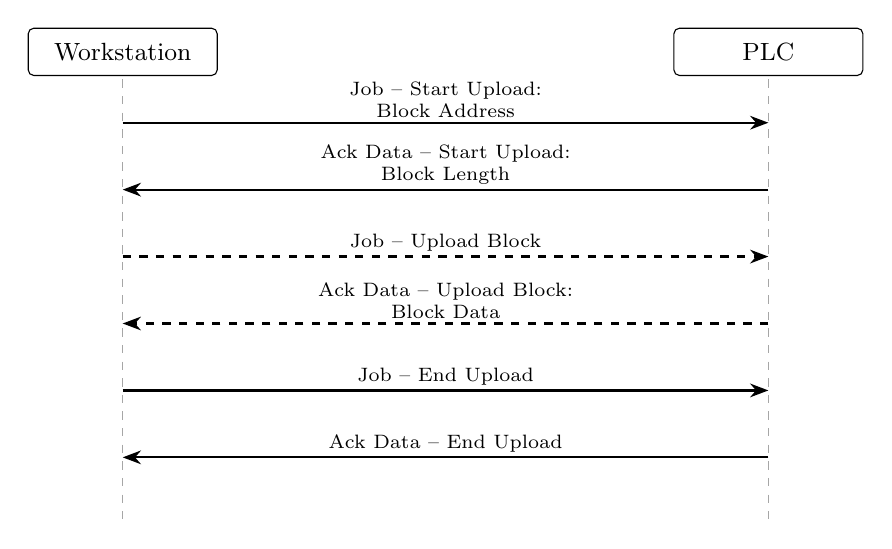
\begin{tikzpicture}[
    font=\small,
    >=Stealth,
    msg/.style={midway, fill=white, inner sep=1.5pt, align=center, font=\scriptsize}
]
    \node[draw, rounded corners=2pt, minimum width=2.4cm, minimum height=0.6cm] (ws) at (0,0) {Workstation};
    \node[draw, rounded corners=2pt, minimum width=2.4cm, minimum height=0.6cm] (plc) at (8.2,0) {PLC};
    \draw[dashed, gray!70] (0,-0.35) -- ++(0,-5.6);
    \draw[dashed, gray!70] (8.2,-0.35) -- ++(0,-5.6);

    \draw[->, thick] (0,-0.9) -- node[msg, above] {Job -- Start Upload:\\Block Address} (8.2,-0.9);
    \draw[->, thick] (8.2,-1.75) -- node[msg, above] {Ack Data -- Start Upload:\\Block Length} (0,-1.75);
    \draw[->, thick, dashed] (0,-2.6) -- node[msg, above] {Job -- Upload Block} (8.2,-2.6);
    \draw[->, thick, dashed] (8.2,-3.45) -- node[msg, above] {Ack Data -- Upload Block:\\Block Data} (0,-3.45);
    \draw[->, thick] (0,-4.3) -- node[msg, above] {Job -- End Upload} (8.2,-4.3);
    \draw[->, thick] (8.2,-5.15) -- node[msg, above] {Ack Data -- End Upload} (0,-5.15);
\end{tikzpicture}%
}

\newcommand{\SSevenDownloadSequence}{%
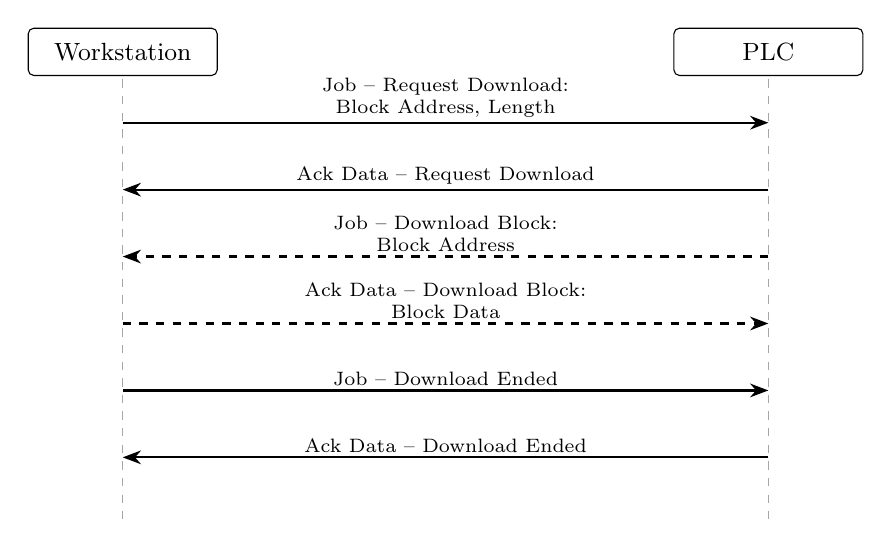
\begin{tikzpicture}[
    font=\small,
    >=Stealth,
    msg/.style={midway, fill=white, inner sep=1.5pt, align=center, font=\scriptsize}
]
    \node[draw, rounded corners=2pt, minimum width=2.4cm, minimum height=0.6cm] (ws) at (0,0) {Workstation};
    \node[draw, rounded corners=2pt, minimum width=2.4cm, minimum height=0.6cm] (plc) at (8.2,0) {PLC};
    \draw[dashed, gray!70] (0,-0.35) -- ++(0,-5.6);
    \draw[dashed, gray!70] (8.2,-0.35) -- ++(0,-5.6);

    \draw[->, thick] (0,-0.9) -- node[msg, above] {Job -- Request Download:\\Block Address, Length} (8.2,-0.9);
    \draw[->, thick] (8.2,-1.75) -- node[msg, above] {Ack Data -- Request Download} (0,-1.75);
    \draw[->, thick, dashed] (8.2,-2.6) -- node[msg, above] {Job -- Download Block:\\Block Address} (0,-2.6);
    \draw[->, thick, dashed] (0,-3.45) -- node[msg, above] {Ack Data -- Download Block:\\Block Data} (8.2,-3.45);
    \draw[->, thick] (0,-4.3) -- node[msg, above] {Job -- Download Ended} (8.2,-4.3);
    \draw[->, thick] (8.2,-5.15) -- node[msg, above] {Ack Data -- Download Ended} (0,-5.15);
\end{tikzpicture}%
}


Hình~\ref{fig:s7-upload-sequence} tóm tắt trình tự trao đổi bản tin Upload S7comm giữa máy trạm kỹ thuật và PLC.

\begin{figure}[htbp]
    \centering
    \SSevenUploadSequence
    \caption{Trình tự Upload S7comm (các pha Job và Ack Data)}
    \label{fig:s7-upload-sequence}
\end{figure}


\begin{enumerate}
    \item \textbf{Start Upload}: Máy client gửi lệnh để yêu cầu PLC trả về chương trình điều khiển nó đang chạy (Job Start Upload) và PLC phản hồi lại yêu cầu đó (Ack Data Start Upload). Command này bao gồm các trường theo thứ tự:
\end{enumerate}


\begin{table}[H]
    \centering
    \footnotesize
    \begin{tabular}{|l|l|l|}
        \hline
        \textbf{Trường} & \textbf{Job Start Upload} & \textbf{Ack Data Start Upload} \\
        \hline
        `Function Code` (1 byte) & Cố định `0x1d` & Same \\
        \hline
        `Function Status` (1 byte) & - & - \\
        \hline
        Không rõ (2 bytes) & `0x0000` & `0x0100` \\
        \hline
        `Session ID` (4 bytes) & - & Định danh cho mỗi phiên upload, được PLC trả về, dùng trong các command sau suốt một phiên Upload \\
        \hline
        Tên tùy thuộc & `Filename Length` (1 byte) theo sau đó là `Filename` chỉ định tên block cần lấy về & `Length String Length` (1 byte) theo sau đó là `Length String` là một số decimal cho biết độ dài của block mà PLC sẽ trả về trong phần data của gói tin phản hồi sau đó \\
        \hline
    \end{tabular}
\end{table}


    \texttt{Filename} là cách định danh một block như sau:


\begin{verbatim}
    ------------------------------------------------------------------------------------------------------------------
    |  1 char - File identifier  |  2 chars - Block type | 5 chars - Block number | 1 char - Destination file system |
    ------------------------------------------------------------------------------------------------------------------
\end{verbatim}


    Với:


\begin{itemize}
    \item \texttt{File identifier} luôn là \texttt{\_}
    \item \texttt{Block type} là một trong các loại block đã nêu
\end{itemize}


\begin{table}[H]
    \centering
    \footnotesize
    \begin{tabular}{|l|l|}
        \hline
        \textbf{Hex} & \textbf{Block type} \\
        \hline
        0x08 & OB \\
        \hline
        0x0a & DB \\
        \hline
        0x0b & SDB \\
        \hline
        0x0c & FC \\
        \hline
        0x0d & SFC \\
        \hline
        0x0e & FB \\
        \hline
        0x0f & SFB \\
        \hline
    \end{tabular}
\end{table}


\begin{itemize}
    \item \texttt{Block number} là số hiệu của block
    \item \texttt{Destination file system} bao gồm \texttt{A} cho Active file system hoặc \texttt{P} cho Passive file system. Block được copy vào active file system sẽ được thực thi ngay khi PLC hoạt động, còn block được copy vào passive file system sẽ cần phải active trước khi được thực thi.
\end{itemize}


    Ví dụ \texttt{\_0800001P} là block OB có số hiệu 1 được copy vào passive file system.


\begin{enumerate}
    \item \textbf{Upload Block}: Sau khi nhận được Start Upload, máy client sẽ gửi lệnh Upload Block để yêu cầu PLC trả về một block dữ liệu của chương trình điều khiển. PLC sẽ trả về block dữ liệu đó trong phần data của gói tin phản hồi. Command này bao gồm các trường theo thứ tự
\end{enumerate}


\begin{table}[H]
    \centering
    \footnotesize
    \begin{tabular}{|l|l|l|}
        \hline
        \textbf{Trường} & \textbf{Job Upload Block} & \textbf{Ack Data Upload Block} \\
        \hline
        `Function Code` (1 byte) & Cố định `0x1e` & Same \\
        \hline
        `Function Status` (1 byte) & - & `0x01` nếu còn nhiều block cần upload, `0x00` nếu đã hết block cần upload \\
        \hline
        Không rõ (2 bytes) & `0x0000` & `0x0000` \\
        \hline
        `Session ID` (4 bytes) & Dùng sessionID đã có & Same \\
        \hline
        `Data` & - & Chữa code chương trình điều khiển, bao gồm `Length` (2 bytes) cho biết độ dài của phần data này, cố định `0x00fb`, `Block Data` chứa dữ liệu của block cần upload. Dữ liệu này ở dạng ASCII \\
        \hline
    \end{tabular}
\end{table}


\begin{enumerate}
    \item \textbf{End Upload}: Khi đã nhận đủ dữ liệu theo trường \texttt{Length String} của gói tin ACK Start Upload, máy client sẽ gửi lệnh End Upload để kết thúc phiên upload. PLC sẽ phản hồi lại yêu cầu đó để xác nhận đã kết thúc phiên upload thành công. Command này bao gồm các trường theo thứ tự:
\end{enumerate}


\begin{table}[H]
    \centering
    \footnotesize
    \begin{tabular}{|l|l|l|}
        \hline
        \textbf{Trường} & \textbf{Job End Upload} & \textbf{Ack Data End Upload} \\
        \hline
        `Function Code` (1 byte) & Cố định `0x1f` & Same \\
        \hline
    \end{tabular}
\end{table}


\subsubsection{Download}

Hình~\ref{fig:s7-download-sequence} tóm tắt trình tự trao đổi bản tin Download S7comm.

\begin{figure}[htbp]
    \centering
    \SSevenDownloadSequence
    \caption{Trình tự Download S7comm (các pha Job và Ack Data)}
    \label{fig:s7-download-sequence}
\end{figure}


\begin{enumerate}
    \item \textbf{Start Download}: Máy client gửi lệnh để yêu cầu PLC chuẩn bị nhận chương trình điều khiển mới (Job Request Download) và PLC phản hồi lại yêu cầu đó (Ack Data Request Download). Gói tin Job Request Download có 2 trường mới là \texttt{Block Length} cho biết độ dài của block dữ liệu mà máy client sẽ gửi, \texttt{Payload Length} cũng thể nhưng không tính độ dài của block header
\end{enumerate}



\begin{enumerate}
    \item \textbf{Download Block}: PLC chủ động gửi request để yêu cầu máy client gửi block dữ liệu của chương trình điều khiển mới. Máy client sẽ gửi block dữ liệu đó trong phần data của gói tin phản hồi.
\end{enumerate}


Các trường thông tin còn lại y hệt như trong phần Upload. Chỉ có lưu ý trong quá trình Download, \texttt{Session ID} luôn là \texttt{0x00000000}, nó không được sử dụng, thay vào đó, trong Download thì sử dụng \texttt{Filename} để định danh trong một session Download.

Lưu lượng chuyển block trực tiếp không thu được trong lab do giới hạn môi trường mô phỏng (OpenPLC nạp qua REST, S7-1500 dùng S7comm-plus trên PLCSIM Advanced). Các lần thử, quan sát trên Wireshark và nguồn PCAP tham chiếu dùng cho luật phát hiện được trình bày ở Phụ lục~\ref{app:upload-download-traffic}.

\subsection{Mô phỏng tấn công Stuxnet (Man-in-the-Middle)}
\label{sec:stuxnet_mitm_sim}

Stuxnet, được công bố rộng rãi từ năm 2010, là một trong các sự cố malware nhắm vào hệ thống điều khiển công nghiệp được biết đến nhiều nhất. Mã độc lây lan trên mạng máy trạm kỹ thuật Windows, sửa logic trên PLC Siemens S7-300 điều khiển máy ly tâm khí tốc độ cao, đồng thời gửi dữ liệu giả mạo tới WinCC khiến vận hành viên vẫn thấy thông số bình thường trong khi quy trình vật lý đã bị tổn hại.

Trong chiến dịch thực tế, Stuxnet đạt được điều này bằng cách hook thư viện giao tiếp Step~7 trên máy trạm kỹ thuật. Đồ án tái hiện cùng hậu quả vận hành ở tầng giao thức S7comm trên lab ở Hình~\ref{fig:lab-topology}: kẻ tấn công ghi đè setpoint trên PLC, đồng thời man-in-the-middle khôi phục giá trị hiển thị trên HMI. Các đoạn dưới tóm tắt chuỗi tấn công lịch sử theo tài liệu công khai; phần cấu hình lab OpenPLC/FUXA và các ảnh chụp gói tin trình bày ngay sau đó.

\paragraph{Chuỗi tấn công lịch sử.}

\begin{enumerate}
    \item \textbf{Lây nhiễm trong windows}: Được lây nhiễm vào một máy tính trong mạng nội bộ thông qua USB do một gián điệp để lại. Sau đó, nó lan tiếp trong mạng nội bộ thông qua 4 lỗ hổng Zero-day  của Windows và gửi thông tin về các máy chủ Command and Control (C\&C) của kẻ tấn công [[1]].
\end{enumerate}



\begin{enumerate}
    \item \textbf{Lây nhiễm vào phần mềm (*)Siemens Step 7}: Tại mỗi máy tính windows, nó quét để truy tìm phần mềm \textbf{Siemens Step 7}. Nó can thiệp vào thư viện giao tiếp \texttt{s7otbxdx.dll} của Step7 để chặn và sửa luồng trao đổi giữa phần mềm Step 7 và PLC:
\end{enumerate}



Normal communications between Step 7 and a Siemens PLC

Hình~\ref{fig:stuxnet_mitm_sim-image-9} minh họa giao tiếp bình thường giữa Step 7 và PLC Siemens.

\begin{figure}[H]
    \centering
    
\includegraphics[width=0.85\textwidth]{../attacks/stuxnet_mitm_sim/image-9.png}
    \caption{Giao tiếp bình thường giữa Step 7 và PLC Siemens}
    \label{fig:stuxnet_mitm_sim-image-9}
\end{figure}

Stuxnet hijacking communication between Step 7 software and a Siemens PLC

Hình~\ref{fig:stuxnet_mitm_sim-image-10} minh họa stuxnet chiếm quyền giao tiếp giữa Step 7 và PLC Siemens.

\begin{figure}[H]
    \centering
    
\includegraphics[width=0.85\textwidth]{../attacks/stuxnet_mitm_sim/image-10.png}
    \caption{Stuxnet chiếm quyền giao tiếp giữa Step 7 và PLC Siemens}
    \label{fig:stuxnet_mitm_sim-image-10}
\end{figure}


    Về bản chất, đây là một kiểu man-in-the-middle ở tầng phần mềm


\begin{enumerate}
    \item \textbf{Can thiệp vào quá trình điều khiển máy ly tâm khí}: Stuxnet can thiệp vào quá trình điều khiển máy ly tâm khí bằng cách sửa đổi code trong PLC để tăng tốc độ vòng quay của máy ly tâm lên mức cao hơn bình thường. Cụ thể, Stuxnet can thiệp vào Step7 để gửi code độc hại nhằm tăng tốc độ vòng quay đến PLC -> PLC thực thi code, gửi tín hiệu điều khiển đến thiết bị biến tần (VFD Variable Frequency Drive) -> biến tần điều chỉnh tốc độ vòng quay của máy ly tâm -> làm hỏng máy ly tâm.
\end{enumerate}


Hình~\ref{fig:stuxnetmitmsimimage11png} minh họa chuỗi tấn công Stuxnet tác động máy ly tâm qua biến tần.

\begin{figure}[H]
    \centering
    
\includegraphics[width=0.9\textwidth]{../attacks/stuxnet_mitm_sim/image-11.png}
    \caption{Chuỗi tấn công Stuxnet tác động máy ly tâm qua biến tần}
    \label{fig:stuxnetmitmsimimage11png}
\end{figure}


    Đồng thời, Stuxnet cũng can thiệp vào đầu ra của PLC để gửi phần mềm HMI WinCC đọc dữ liệu sai lệch về tình trạng của máy ly tâm, khiến các kỹ sư không nhận ra rằng máy ly tâm đang bị hư hại.



Tuy nhiên điều tinh vi ở đây là Stuxnet chọn lọc các mục tiêu rất kỹ càng. Nếu mục tiêu không thỏa mãn yêu cầu, Stuxnet sẽ ngủ đông để giảm thiểu sự hiện diện của mình. Nó chỉ tấn công vào các PLC điều khiển biến tần có thông số:


\begin{itemize}
    \item Thuộc dòng Siemens S7-300
\end{itemize}


\begin{itemize}
    \item Nhà sản xuất biến tần là Vacon (Finland)hoặc Fararo Paya (Iran)
\end{itemize}


\begin{itemize}
    \item Tần số vận hành nằm trong khoảng \textbf{807} Hz đến \textbf{1210} Hz. Do đây là tốc độ quay lớn hơn nhiều so với tốc độ của hầu hết các máy công nghiệp, trừ máy ly tâm khí.
\end{itemize}


Khi đủ điều kiện, Stuxnet thay đổi tần số đầu ra trong các giai đoạn ngắn để làm rối loạn hoạt động của hệ thống, với các mức thường được nhắc đến là 1410 Hz, 2 Hz và 1064 Hz. Với cách này, nó làm thay đổi tốc độ quay của máy ly tâm và có thể gây hư hại vật lý, trong khi dữ liệu giám sát vẫn bị che giấu.

\textit{Trong mô phỏng tấn công của đồ án này, để phù hợp với giới hạn về thời gian và nguồn lực, chúng tôi sẽ mô phỏng đơn giản hóa kịch bản tấn công man-in-the-middle ở trên tầng giao thức mạng thay vì tại dll như thực tế Stuxnet đã làm.}


\textbf{(*)} \textit{Tia Portal là một bộ phần mềm độc quyền của Siemens để làm việc với các dòng PLC của hãng (S7-300, S7-400, S7-1200, S7-1500), bao gồm: STEP 7 dùng để lập trình và cấu hình cho các dòng PLC, WinCC dùng để thiết kế HMI/SCADA, S7- PLCSIM / S7 PLCSIM Advanced dùng để mô phỏng hoạt động của PLC trên máy tính mà không cần phần cứng thực tế, Startdrive dùng để cấu hình biến tần, động cơ.}


\noindent\textbf{Mô phỏng tấn công.}\par
\medskip

\begin{verbatim}
![alt text](<Stuxnet (1).svg>)
\end{verbatim}


\textit{Mục tiêu của tấn công là làm thay đổi giá trị của một biến nằm trong datablock của PLC, từ đó làm thay đổi hành vi của hệ thống điều khiển. Đồng thời can thiệp vào quá trình gửi dữ liệu để HMI không nhận ra sự thay đổi này.}


\subsubsection{Thiết lập PLC}


Import dự án vào OpenPLC Editor với thư mục này (\url{./plc_server_code/}). Chương trình đang chạy trên PLC có dạng như sau


\begin{itemize}
    \item Với cấu hình datablock như sau để làm biến đầu vào (DB1) và ra (DB2) cho PLC:
\end{itemize}


Hình~\ref{fig:stuxnet_mitm_sim-image-1} minh họa cấu hình datablock đầu vào (DB1) và đầu ra (DB2) cho PLC.

\begin{figure}[H]
    \centering
    
\includegraphics[width=0.85\textwidth]{../attacks/stuxnet_mitm_sim/image-1.png}
    \caption{Cấu hình datablock đầu vào (DB1) và đầu ra (DB2) cho PLC}
    \label{fig:stuxnet_mitm_sim-image-1}
\end{figure}

Khai báo 2 datablock do mỗi datablock trong OpenPLC chỉ cho phép 1 kiểu dữ liệu


\begin{itemize}
    \item Khai báo tag và chương trình logic (viết dưới dạng Structured Text). Chương trình mô phỏng lại tốc độ quay của động cơ dao động quanh mốc \texttt{iSetpoint} được chỉ định bằng \texttt{1200}:
\end{itemize}


Hình~\ref{fig:stuxnet_mitm_sim-image-2} minh họa khai báo tag và chương trình logic dạng Structured Text.

\begin{figure}[H]
    \centering
    
\includegraphics[width=0.85\textwidth]{../attacks/stuxnet_mitm_sim/image-2.png}
    \caption{Khai báo tag và chương trình logic dạng Structured Text}
    \label{fig:stuxnet_mitm_sim-image-2}
\end{figure}

Khai báo tag và chương trình logic (viết dưới dạng Structured Text)


    Gồm các tags (Giống dạng binding variables trong IT):


\begin{itemize}
    \item \texttt{iSimSpeed}: tốc độ thực tế máy đang quay, nằm ở \texttt{DB1}, lấy 2 Byte từ offset 0
    \item \texttt{iSetpoint}: tốc độ ngưỡng để máy quay dao động quanh giá trị này, nằm ở \texttt{DB1}, lấy 2 Byte từ offset 2
    \item \texttt{iCounter}: Dùng để tạo dao động mô phỏng.
    \item \texttt{bCentrifugeStatus}: trạng thái hoạt động của máy ly tâm với 0 là bình thường, 1 là quá tốc độ, nằm ở \texttt{DB2}, lấy 1 Byte từ offset 0. Ở đây mô phỏng khi tốc độ quay vượt quá 1500 Hz thì máy ly tâm bị hư hại.
\end{itemize}




\subsubsection{Thiết lập HMI}


Import dự án vào FUXA với thư mục này (\url{./hmi/fuxa_hmi_design.json}):


Hình~\ref{fig:stuxnet_mitm_sim-image-8} minh họa import dự án FUXA HMI và cấu hình tag.

\begin{figure}[H]
    \centering
    
\includegraphics[width=0.85\textwidth]{../attacks/stuxnet_mitm_sim/image-8.png}
    \caption{Import dự án FUXA HMI và cấu hình tag}
    \label{fig:stuxnet_mitm_sim-image-8}
\end{figure}

Khai báo các HMI tags tương ứng với các PLC tags cần giám sát


Giao diện HMI, hiện tại máy đang hoạt động quanh mức 1200 nên sẽ hiển thị màu xanh


Trong Debugger của OpenPLC Editor cũng hiển thị thông tin tương tự:


Hình~\ref{fig:stuxnet_mitm_sim-image-17} minh họa thông tin tương tự trên OpenPLC Editor Debugger.

\begin{figure}[H]
    \centering
    
\includegraphics[width=0.85\textwidth]{../attacks/stuxnet_mitm_sim/image-17.png}
    \caption{Thông tin tương tự trên OpenPLC Editor Debugger}
    \label{fig:stuxnet_mitm_sim-image-17}
\end{figure}

Thông tin tương tự trong Debugger của OpenPLC Editor


\textit{Nên bật OpenPLC Editor nên để kiểm tra lại xem chương trình đã được nạp vào PLC chưa trước khi kết nối tới HMI hay đọc ghi vào PLC}


Thu thập gói tin trên máy HMI thấy giao tiếp giữa HMI và PLC là sự lặp đi lặp lại của 2 cặp request-response sau:


\begin{itemize}
    \item Cặp đầu tiên là request yêu cầu đọc 4 byte tại DB1 tại bit 0 của byte 0, tức ứng với biến \texttt{iSimSpeed} và \texttt{iSetpoint}:
\end{itemize}


Hình~\ref{fig:stuxnet_mitm_sim-image-4} minh họa yêu cầu đọc 4 byte tại DB1 từ bit 0 byte 0 cho \texttt{iSimSpeed} và \texttt{iSetpoint}.

\begin{figure}[H]
    \centering
    
\includegraphics[width=0.85\textwidth]{../attacks/stuxnet_mitm_sim/image-4.png}
    \caption{Yêu cầu đọc 4 byte tại DB1 từ bit 0 byte 0 cho \texttt{iSimSpeed} và \texttt{iSetpoint}}
    \label{fig:stuxnet_mitm_sim-image-4}
\end{figure}

Request yêu cầu đọc 4 byte tại DB1 tại bit 0 của byte 0, tức ứng với biến \texttt{iSimSpeed} và \texttt{iSetpoint}




Hình~\ref{fig:stuxnet_mitm_sim-image-5} minh họa phản hồi trả về giá trị \texttt{iSimSpeed} và \texttt{iSetpoint}.

\begin{figure}[H]
    \centering
    
\includegraphics[width=0.85\textwidth]{../attacks/stuxnet_mitm_sim/image-5.png}
    \caption{Phản hồi trả về giá trị \texttt{iSimSpeed} và \texttt{iSetpoint}}
    \label{fig:stuxnet_mitm_sim-image-5}
\end{figure}

Response trả về giá trị của biến \texttt{iSimSpeed} và \texttt{iSetpoint}


    Biến \texttt{iSimSpeed} là \texttt{042d} do nó nằm ở trước trong cấu hình các PLC tags, biến \texttt{iSetpoint} là \texttt{04b0}. S7 dùng Little Endian, nên giá trị \texttt{042d} tương ứng với \texttt{1069} và \texttt{04b0} tương ứng với \texttt{1200}.


\begin{itemize}
    \item Cặp thứ hai là request yêu cầu đọc 1 byte tại DB2 tại bit 0 của byte 0, tức ứng với biến \texttt{bCentrifugeStatus}:
\end{itemize}


Hình~\ref{fig:stuxnet_mitm_sim-image-6} minh họa yêu cầu đọc 1 byte tại DB2 từ bit 0 byte 0 cho \texttt{bCentrifugeStatus}.

\begin{figure}[H]
    \centering
    
\includegraphics[width=0.85\textwidth]{../attacks/stuxnet_mitm_sim/image-6.png}
    \caption{Yêu cầu đọc 1 byte tại DB2 từ bit 0 byte 0 cho \texttt{bCentrifugeStatus}}
    \label{fig:stuxnet_mitm_sim-image-6}
\end{figure}

Request yêu cầu đọc 1 byte tại DB2 tại bit 0 của byte 0, tức ứng với biến \texttt{bCentrifugeStatus}


Hình~\ref{fig:stuxnet_mitm_sim-image-7} minh họa phản hồi trả về \texttt{bCentrifugeStatus}; hiện tại bằng 0 (vận hành bình thường).

\begin{figure}[H]
    \centering
    
\includegraphics[width=0.85\textwidth]{../attacks/stuxnet_mitm_sim/image-7.png}
    \caption{Phản hồi trả về \texttt{bCentrifugeStatus}; hiện tại bằng 0 (vận hành bình thường)}
    \label{fig:stuxnet_mitm_sim-image-7}
\end{figure}

Response trả về giá trị của biến \texttt{bCentrifugeStatus}. Hiện đang là 0 tức máy đang hoạt động bình thường


\subsubsection{Attacker}


Từ máy tấn công sẽ làm đồng thời:


\begin{enumerate}
    \item \textbf{Tạo một lệnh ghi để ghi} giá trị của một biến nằm trong Datablock của PLC sử dụng thư viện Snap 7 hoặc S7 Comm của Python. Việc ghi này dễ dàng do giao thức S7 không có cơ chế xác thực. Ở đây sẽ chỉnh sửa giá trị biến \texttt{Setpoint} nằm ở vị trí \texttt{DB1.DBW2} từ \texttt{1200} thành \texttt{2000}. Script tại đây (Bản dùng thư viện Snap7) (\url{./attacker/test_readwrite_db_via_snap7.py}) hoặc đây (Bản dùng thư viện S7 Comm) (\url{./attacker/test_readwrite_db_via_pythonS7comm.py}). Output:
\end{enumerate}


\begin{verbatim}
    Current Speed  | Setpoint Speed    | Centrifuge Status
    --------------------------------------------------
    b'\x03\xc1'    |    b'\x04\xb0'    |    b'\x00'
    b'\x07\xe4'    |    b'\x07\xd0'    |    b'\x01'
\end{verbatim}


    \texttt{iSetpoint} từ \texttt{1200} (0x04b0) thành \texttt{2000} (0x07d0) và khi này trạng thái \texttt{bCentrifugeStatus} từ \texttt{0} thành \texttt{1}.  Nếu như chưa chạy script can thiệp thì trên HMI sẽ thấy máy đang dao động quanh mức 2000:


Hình~\ref{fig:stuxnet_mitm_sim-image-14} minh họa máy dao động quanh 2000, hiển thị đỏ vì vượt ngưỡng 1500 Hz.

\begin{figure}[H]
    \centering
    
\includegraphics[width=0.85\textwidth]{../attacks/stuxnet_mitm_sim/image-14.png}
    \caption{Máy dao động quanh 2000, hiển thị đỏ vì vượt ngưỡng 1500 Hz}
    \label{fig:stuxnet_mitm_sim-image-14}
\end{figure}

Máy đang dao động quanh mức 2000, hiển thị màu đỏ do quá mốc 1500 Hz



Hình~\ref{fig:stuxnet_mitm_sim-image-15} minh họa gói PLC-to-HMI cho thấy \texttt{iSetpoint} đổi thành \texttt{2000} (0x07d0).

\begin{figure}[H]
    \centering
    
\includegraphics[width=0.85\textwidth]{../attacks/stuxnet_mitm_sim/image-15.png}
    \caption{Gói PLC-to-HMI cho thấy \texttt{iSetpoint} đổi thành \texttt{2000} (0x07d0)}
    \label{fig:stuxnet_mitm_sim-image-15}
\end{figure}

Kiểm tra trong các gói tin PLC gửi tới HMI để thấy giá trị của biến \texttt{iSetpoint} đã được thay đổi thành \texttt{2000} (0x07d0)


    Tấn công thay đổi giá trị của PLC thành công, giờ ta sẽ can thiệp vào giao tiếp giữa HMI và PLC để HMI không nhận ra sự thay đổi này.




\begin{enumerate}
    \item \textbf{Tấn công Man in the middle bằng kỹ thuật ARP Spoofing} giữa cổng của Router (\texttt{.60.1}) và HMI (\texttt{.60.10}) thông qua tool \textbf{Bettercap}:
\end{enumerate}



\begin{verbatim}
    # Run on attacker machine
    sudo bettercap -iface ens33 

    # Scan network for devices
    net.probe on

    # Show network devices
    net.show
\end{verbatim}


    Đảm bảo đã Bettercap đã thu được thông tin của tất cả các thiết bị trong mạng:


\begin{verbatim}
    +---------------+-------------------+---------+--------------+-------+--------+----------+
    |     IP ^      |        MAC        |  Name   |    Vendor    | Sent  | Recvd  |   Seen   |
    +---------------+-------------------+---------+--------------+-------+--------+----------+
    | 192.168.60.20 | 00:0c:29:a6:c0:b0 | ens33   | VMware, Inc. | 0 B   | 0 B    | 14:52:24 |
    | 192.168.60.1  | 00:0c:29:f1:b8:5e | gateway | VMware, Inc. | 816 B | 0 B    | 14:52:24 |
    |               |                   |         |              |       |        |          |
    | 192.168.60.10 | 00:0c:29:2f:0d:bb |         | VMware, Inc. | 16 kB | 8.3 kB | 14:53:43 |
    +---------------+-------------------+---------+--------------+-------+--------+----------+
\end{verbatim}


\begin{verbatim}
    # Specify IP of Router gateway and HMI as targets
    set arp.spoof.targets 192.168.60.1, 192.168.60.10
    
    # Enable internal ARP spoofing
    set arp.spoof.internal true
    # Enable full duplex ARP spoofing since we need to ensure HMI -> PLC direction is still working
    set arp.spoof.fullduplex true
    
    # Start ARP spoofing
    arp.spoof on
\end{verbatim}


    Khi này trên HMI bắt gói tin sẽ thấy xen kẽ các gói tin của S7 và các gói ARP Spoofing:


Hình~\ref{fig:stuxnet_mitm_sim-image-13} minh họa gói S7comm xen kẽ với gói ARP spoofing.

\begin{figure}[H]
    \centering
    
\includegraphics[width=0.85\textwidth]{../attacks/stuxnet_mitm_sim/image-13.png}
    \caption{Gói S7comm xen kẽ với gói ARP spoofing}
    \label{fig:stuxnet_mitm_sim-image-13}
\end{figure}

Gói tin S7comm và ARP Spoofing xen kẽ nhau


\begin{enumerate}
    \item \textbf{Chỉnh sửa gói tin S7comm} được gửi từ PLC tới HMI để thay đổi giá trị \texttt{Setpoint} từ \texttt{2000} thành \texttt{1200}. Sau khi Bettercap đã redirect được gói tin giữa Router gateway và Router, đẩy các gói tin này vào NFQUEUE của OS (Vì ta muốn xử lý các gói tin thay vì để OS tự động chuyển tiếp) và sử dụng một script Python để lấy gói tin từ NFQUEUE (thông qua thư viện \texttt{NetfilterQueue}), parse gói tin S7comm, tìm đến vị trí chứa giá trị \texttt{Setpoint} ở \texttt{DB1.DBW2} và sửa giá trị này từ \texttt{2000} thành \texttt{1200} trước khi đẩy gói tin trở lại NFQUEUE để tiếp tục được chuyển đi. Script tại đây (\url{./attacker/mitm/s7_intercept.py}).
\end{enumerate}


Hình~\ref{fig:stuxnet_mitm_sim-image-18} minh họa tấn công thành công: tốc độ thực tế trên 1500 Hz (đỏ) nhưng Setpoint vẫn hiển thị 1200.

\begin{figure}[H]
    \centering
    
\includegraphics[width=0.85\textwidth]{../attacks/stuxnet_mitm_sim/image-18.png}
    \caption{Tấn công thành công: tốc độ thực tế trên 1500 Hz (đỏ) nhưng Setpoint vẫn hiển thị 1200}
    \label{fig:stuxnet_mitm_sim-image-18}
\end{figure}

Tấn công thành công khi thực tế máy đang chạy ở mức > 1500 Hz (màu đỏ), nhưng Setpoint vẫn hiển thị ở mức 1200


Kiểm tra các gói tin:


Hình~\ref{fig:stuxnet_mitm_sim-image-28} minh họa gói PLC-to-HMI với \texttt{iSetpoint} giả mạo = 1200 (\texttt{04b0}).

\begin{figure}[H]
    \centering
    
\includegraphics[width=0.85\textwidth]{../attacks/stuxnet_mitm_sim/image-28.png}
    \caption{Gói PLC-to-HMI với \texttt{iSetpoint} giả mạo = 1200 (\texttt{04b0})}
    \label{fig:stuxnet_mitm_sim-image-28}
\end{figure}

Giá trị \texttt{iSetpoint} trên gói tin tới HMI đang là 1200 (04b0)


Hình~\ref{fig:stuxnet_mitm_sim-image-29} minh họa gói PLC-to-HMI với \texttt{bCentrifugeStatus} = 01 (quá tốc).

\begin{figure}[H]
    \centering
    
\includegraphics[width=0.85\textwidth]{../attacks/stuxnet_mitm_sim/image-29.png}
    \caption{Gói PLC-to-HMI với \texttt{bCentrifugeStatus} = 01 (quá tốc)}
    \label{fig:stuxnet_mitm_sim-image-29}
\end{figure}

Giá trị \texttt{bCentrifugeStatus} trên gói tin tới HMI 01



Hình~\ref{fig:stuxnet_mitm_sim-image-3} minh họa openPLC Editor debugger cho thấy tốc độ quá trình thực tế gần 2000.

\begin{figure}[H]
    \centering
    
\includegraphics[width=0.85\textwidth]{../attacks/stuxnet_mitm_sim/image-3.png}
    \caption{OpenPLC Editor debugger cho thấy tốc độ quá trình thực tế gần 2000}
    \label{fig:stuxnet_mitm_sim-image-3}
\end{figure}

Kiểm tra debugger của OpenPLC Editor cũng cho thấy thực tế máy đang chạy giao động quanh mốc 2000


\subsubsection{Phân tích tấn công}


Phần khó nhất của cuộc tấn công này là làm sao sửa đổi gói tin rồi chuyển tiếp lại được. Để đảm bảo tốc độ, ở đây sử dụng phương pháp ARP Spoofing bằng Bettercap để redirect gói tin đến máy Attacker, tại đây, gói tin sẽ được đẩy vào NFQUEUE để Python app gọi lên xử lý thay vì để OS Kernel tự động forward gói tin đi. 


\textit{Một phần vì Bettercap chỉ cung cấp khả năng chỉnh sửa gói tin khi intercept bằng Javascript mà ngôn ngữ này lại không phù hợp để viết bộ S7 Parser nên mới phải làm cách này}


\begin{verbatim}
# 1. Bật IP Forwarding
subprocess.run("sysctl -w net.ipv4.ip_forward=1 > /dev/null", shell=True)

# 2. Tắt RP Filter (Tránh rớt gói tin chiều về từ Router)
# Tránh kernel tự động drop gói tin lạ -> Cho phép gói tin từ PLC về được phép qua
subprocess.run("sysctl -w net.ipv4.conf.all.rp_filter=0 > /dev/null", shell=True)
subprocess.run("sysctl -w net.ipv4.conf.default.rp_filter=0 > /dev/null", shell=True)
subprocess.run(f"sysctl -w net.ipv4.conf.{INTERFACE}.rp_filter=0 > /dev/null", shell=True)

# 3. Thêm Route tới dải PLC thông qua Gateway thật
# Không có dòng này sẽ gây lỗi mất kết nối ngay lập tức trên HMI khi nó gửi yêu
# cầu read var tới PLC
print(f"[*] Thêm tuyến đường tới {PLC_NET} qua {GATEWAY}...")
subprocess.run(f"route add -net {PLC_NET} gw {GATEWAY} 2>/dev/null", shell=True)

# 4. Cấu hình Iptables
print("[*] Đang thiết lập Iptables NFQUEUE...")
subprocess.run("iptables -F", shell=True)               # Xóa sạch filter table
subprocess.run("iptables -t mangle -F", shell=True)      # Xóa sạch mangle table
subprocess.run("iptables -P FORWARD ACCEPT", shell=True) # Đảm bảo forward không bị chặn

# Bẫy traffic S7 (Port 102) vào Queue
# Để thay vì Kernel tự động drop gói tin, python app sẽ xử lý gói tin và chuyển tiếp lại
subprocess.run(f"iptables -t mangle -A FORWARD -p tcp --dport 102 -j NFQUEUE --queue-num {QUEUE_NUM}", shell=True)
subprocess.run(f"iptables -t mangle -A FORWARD -p tcp --sport 102 -j NFQUEUE --queue-num {QUEUE_NUM}", shell=True)

# Chặn gói RST tự phát từ Kernel (Tránh Disconnected)
# Kernel sẽ tự gửi RST (reset connection) nếu nhận gói từ port nó không biết
subprocess.run("iptables -I OUTPUT -p tcp --tcp-flags RST RST -j DROP", shell=True)
\end{verbatim}


Sau khi đã có được gói tin cần tiến hành chỉnh sửa. Cấu trúc của gói tin S7 như sau:


Hình~\ref{fig:iemensS7protocolstackpng} minh họa ngăn xếp giao thức Siemens S7.

\begin{figure}[H]
    \centering
    
\includegraphics[width=0.9\textwidth]{../attacks/stuxnet_mitm_sim/Siemens_S7_protocol_stack.png}
    \caption{Ngăn xếp giao thức Siemens S7}
    \label{fig:iemensS7protocolstackpng}
\end{figure}


Với:


\begin{itemize}
    \item \texttt{TPKT Header}: Cố định là 4 byte như đã trình bày trong phần lý thuyết về giao thức S7.

Hình~\ref{fig:stuxnet_mitm_sim-image-19} minh họa header TPKT.

\begin{figure}[H]
    \centering
    
\includegraphics[width=0.9\textwidth]{../attacks/stuxnet_mitm_sim/image-19.png}
    \caption{Header TPKT}
    \label{fig:stuxnet_mitm_sim-image-19}
\end{figure}

    \item \texttt{COTP Header}: Cố định là 3 byte như đã trình bày trong phần lý thuyết về giao thức S7.

Hình~\ref{fig:stuxnet_mitm_sim-image-20} minh họa header COTP.

\begin{figure}[H]
    \centering
    
\includegraphics[width=0.9\textwidth]{../attacks/stuxnet_mitm_sim/image-20.png}
    \caption{Header COTP}
    \label{fig:stuxnet_mitm_sim-image-20}
\end{figure}

    \item \texttt{S7 Header}: Byte đầu tiên luôn là \texttt{0x32}, ta dùng byte này để phân biệt gói tin S7comm và các gói tin khác. Ngoài ra trong đây có một trường mà ta cần quan tâm đó chính là \texttt{ROSCTR} - \texttt{ROS Control}, đây là trường quyết định loại lệnh S7comm mà PLC gửi đi. Cụ thể:
    \begin{itemize}
        \item \texttt{0x01}: Job
        \item \texttt{0x02}: Ack
        \item \texttt{0x03}: Ack\_Data
    \end{itemize}
\end{itemize}


    Như trong trường hợp này, quan sát thấy gói tin Read Var Request sẽ có \texttt{ROSCTR} là \texttt{Job}

Hình~\ref{fig:stuxnetmitmsimimage25png} minh họa read Var Request với ROSCTR = Job.

\begin{figure}[H]
    \centering
    
\includegraphics[width=0.9\textwidth]{../attacks/stuxnet_mitm_sim/image-25.png}
    \caption{Read Var Request với ROSCTR = Job}
    \label{fig:stuxnetmitmsimimage25png}
\end{figure}


    còn gói tin Read Var Response sẽ có \texttt{ROSCTR} là \texttt{Ack\_Data}.

Hình~\ref{fig:stuxnetmitmsimimage26png} minh họa read Var Response với ROSCTR = Ack\_Data.

\begin{figure}[H]
    \centering
    
\includegraphics[width=0.9\textwidth]{../attacks/stuxnet_mitm_sim/image-26.png}
    \caption{Read Var Response với ROSCTR = Ack\_Data}
    \label{fig:stuxnetmitmsimimage26png}
\end{figure}


    Mấy trường còn lại trong Header không quan trọng cho dự án này.


\begin{itemize}
    \item Phần \texttt{Param} và \texttt{Data} sẽ tuỳ thuộc vào loại lệnh S7comm đang được sử dụng, ví dụ như Setup Communication, Read Var, Write Var, ...
\end{itemize}


Ở đây chỉ xét tới phần \texttt{Param} và \texttt{Data} của loại lệnh \textbf{Read Var} [[2]]. Đầu tiên là về cách định vị các Var muốn đọc. S7 có 3 cách để định vị các Var:


\begin{itemize}
    \item \textbf{Any-type}: Chỉ rõ \texttt{area} (ví dụ: \texttt{DB}, \texttt{M}, \texttt{I}, \texttt{Q}), \texttt{address} (tức byte nào), kiểu dữ liệu. Ví dụ đọc biến \texttt{DB1.DBX0.0} sẽ có \texttt{area = DB}, \texttt{address = 1} (tức byte thứ 1), kiểu dữ liệu là bit Khi này, cấu trúc của phần \texttt{Param} sẽ là:
\end{itemize}


    Với Read Var \textbf{Request}:


\begin{verbatim}
![alt text](AnyTypeStruct.svg)
\end{verbatim}


\begin{itemize}
    \item \texttt{Function Code}: \texttt{0x04} vì đây là lệnh Read Var (Các kiểu định vị khác như DB-Type, Symbolic cũng giống trường này vì chúng đều thuộc nhóm command đọc ghi biến (\texttt{0x04}/\texttt{0x05}).)
    \item \texttt{Item count}: Số lượng Items có sẽ được chỉ định trong gói tin này (Các kiểu định vị khác như DB-Type, Symbolic cũng giống trường này). Như trong hình là có 2 items.
\end{itemize}


\begin{itemize}
    \item Các kiểu định vị chỉ khác nhau ở phần cấu trúc của \texttt{Request Item}:
    \item \texttt{Spec Type}: Luôn là \texttt{0x12}
    \item \texttt{Length}: Độ dài của Item này
    \item \texttt{Syntax ID}: \texttt{0x10} cho kiểu Any-type, \texttt{0xb0} cho kiểu DB-Type
\end{itemize}


            Ảnh chụp lưu lượng từ Wireshark cho thấy hai bên trong dự án giao tiếp với nhau bằng kiểu Any-type \texttt{0x10}:

Hình~\ref{fig:stuxnetmitmsimimage22png} minh họa địa chỉ Any-type trong lưu lượng bắt được.

\begin{figure}[H]
    \centering
    
\includegraphics[width=0.9\textwidth]{../attacks/stuxnet_mitm_sim/image-22.png}
    \caption{Địa chỉ Any-type trong lưu lượng bắt được}
    \label{fig:stuxnetmitmsimimage22png}
\end{figure}


\begin{itemize}
    \item \texttt{Variable Type}: xác định kiểu dữ liệu và độ dài của biến (thường sử dụng các kiểu dữ liệu S7 như REAL, BIT, BYTE, WORD, DWORD, COUNTER, …).
    \item \texttt{Count}: có thể chọn toàn bộ một mảng các biến có cùng kiểu bằng cách sử dụng một struct item duy nhất. Các biến này phải cùng kiểu, và phải liên tiếp trong bộ nhớ và trường \texttt{Count} xác định kích thước của mảng này. Được đặt là 1 cho việc đọc hoặc ghi một biến duy nhất.
    \item Các trường còn lại xách định địa chỉ muốn đọc, viết theo đúng cấu trúc của Any-type với \texttt{DB Number} (chỉ có khi \texttt{area} là DB) cho datablock muốn đọc, \texttt{Area} cho loại vùng nhớ muốn đọc (DB, M, I, Q), \texttt{Address} cho địa chỉ cụ thể muốn đọc trong vùng nhớ đó. Trường \texttt{Address} 3 byte này encode bit offset theo dạng big-endian.
\end{itemize}


Hình~\ref{fig:stuxnetmitmsimimage21png} minh họa các trường request item kiểu Any-type.

\begin{figure}[H]
    \centering
    
\includegraphics[width=0.9\textwidth]{../attacks/stuxnet_mitm_sim/image-21.png}
    \caption{Các trường request item kiểu Any-type}
    \label{fig:stuxnetmitmsimimage21png}
\end{figure}


    Với Read Var \textbf{Response} tương tự, chỉ thay thế phần \texttt{Request Item} thành \texttt{Data Item}:


\begin{verbatim}
![alt text](ReadVarResponse.svg)
\end{verbatim}


\begin{itemize}
    \item \texttt{Error Code}: \texttt{0xff} cho success
    \item \texttt{Variable Type} và \texttt{Count} giống như Request Item
    \item \texttt{Data}: Trả về dữ liệu cho các Items tương ứng được hỏi trong Request Item.

Hình~\ref{fig:stuxnet_mitm_sim-image-23} minh họa data item trong phản hồi Read Var.

\begin{figure}[H]
    \centering
    
\includegraphics[width=0.9\textwidth]{../attacks/stuxnet_mitm_sim/image-23.png}
    \caption{Data item trong phản hồi Read Var}
    \label{fig:stuxnet_mitm_sim-image-23}
\end{figure}

\end{itemize}



\begin{itemize}
    \item \textbf{DB-Type}: dành riêng cho area DB, ngắn gọn hơn cách trên. Tạm không phân tích vì trong dự án này không sử dụng. Cấu trúc của Request Item và Response Item như sau:
\end{itemize}


Hình~\ref{fig:stuxnetmitmsimimage24png} minh họa request và response item kiểu DB-Type.

\begin{figure}[H]
    \centering
    
\includegraphics[width=0.9\textwidth]{../attacks/stuxnet_mitm_sim/image-24.png}
    \caption{Request và response item kiểu DB-Type}
    \label{fig:stuxnetmitmsimimage24png}
\end{figure}


\begin{itemize}
    \item \textbf{Symbolic}: Thay vì dùng địa chỉ byte, ta có thể dùng tên biến đã được định nghĩa trong chương trình PLC. Ví dụ: \texttt{DB1.CustomProperty1}. Khi này tham số sẽ bao gồm tên biến và kiểu dữ liệu. Cách này chỉ hỗ trợ trên các dòng S7-1200/1500. Tạm không phân tích vì trong dự án này không sử dụng.
\end{itemize}


Lý do cần phân tích cấu trúc gói tin là vì đã thử tìm trên mạng nhưng không có bộ Parser nào cho S7, chỉ duy nhất có một bộ Parser bằng C tại  https://github.com/ricardojoserf/s7-parser. Tuy nhiên nó có một vấn đề là không thể parse được phần \texttt{Data} trong \texttt{Response Item} của gói tin S7, nên dự án đã dựa vào đó để viết lại bộ parser bằng Python và cải tiến thêm để có thể parse được phần \texttt{Data} này. Script tại đây (\url{./attacker/mitm/s7_parser.py}).


Thử nghiệm bộ parser bằng cách chạy trên một file PCAP, chỉ định gói tin cần extract (ở đây là gói tin thứ 9):

\begin{verbatim}
uv run .\s7_parser.py .\wincc_s300_setup-alarm-read-write.pcapng 9
\end{verbatim}


Output:


\begin{verbatim}
Analyzing S7 packet #9:

================================================================================
S7 Protocol Packet Detected
================================================================================

S7 Communication
  Header: (Ack_Data)
    Protocol Id: 0x32
    ROSCTR: Ack_Data (3)
    Redundancy Identification (Reserved): 0x0000
    Protocol Data Unit Reference: 2
    Parameter length: 2
    Data length: 52
    Error class: No error (0x00)
    Error code: 0x00
  Parameter: (Read Var)
    Function: Read Var (0x04)
    Item count: 8
  Data
    Item [1]: (Success)
      Return code: Success (0xff)
      Transport size: BIT (0x03)
      Length: 1
      Data: 01
    Item [2]: (Success)
      Return code: Success (0xff)
      Transport size: REAL (0x07)
      Length: 4
      Data: aabbccdd
    Item [3]: (Success)
      Return code: Success (0xff)
      Transport size: BYTE/WORD/DWORD (0x04)
      Length: 4
      Data: feadbeef
    Item [4]: (Success)
      Return code: Success (0xff)
      Transport size: BYTE/WORD/DWORD (0x04)
      Length: 2
      Data: babe
    Item [5]: (Success)
      Return code: Success (0xff)
      Transport size: BIT (0x03)
      Length: 1
      Data: 01
    Item [6]: (Success)
      Return code: Success (0xff)
      Transport size: BIT (0x03)
      Length: 1
      Data: 01
    Item [7]: (Success)
      Return code: Success (0xff)
      Transport size: OCTET STRING (0x09)
      Length: 2
      Data: 2504
    Item [8]: (Success)
      Return code: Success (0xff)
      Transport size: OCTET STRING (0x09)
      Length: 2
      Data: 0011

================================================================================

\end{verbatim}


Giống với cách gói tin được Parse trong Wireshark:


Hình~\ref{fig:stuxnetmitmsimimage16png} minh họa gói S7 được parse trong Wireshark.

\begin{figure}[H]
    \centering
    
\includegraphics[width=0.9\textwidth]{../attacks/stuxnet_mitm_sim/image-16.png}
    \caption{Gói S7 được parse trong Wireshark}
    \label{fig:stuxnetmitmsimimage16png}
\end{figure}



Bây giờ việc của \texttt{s7\_intercept.py} (\url{./attacker/mitm/s7_intercept.py}) là:

\begin{enumerate}
    \item Lấy các gói tin S7 lên từ NFQUEUE, mỗi gói tin gọi hàm \texttt{process\_packet} để xử lý.

    \item Hàm \texttt{process\_packet} sẽ kiểm tra đây có phải là gói tin S7 comm không bằng cách kiểm tra tuần tự:
    \begin{itemize}
        \item Byte TPKT: \texttt{payload[0] == 0x03};
        \item COTP: \texttt{payload[4] == 0x02};
        \item S7 Header: \texttt{payload[7] == 0x32};
        \item ROSCTR: \texttt{payload[8] == 0x03} (tức gói tin Response từ PLC gửi về HMI).
    \end{itemize}

    \item Nếu là gói tin S7 comm và là gói tin Response từ PLC gửi về HMI, thì tại đây sẽ có 2 trường hợp (ứng với 2 cặp request-response đã đề cập ở đầu):
    \begin{itemize}
        \item Gói tin trả lời cho lệnh đọc 1 bit \texttt{bCentrifugeStatus} tại \texttt{DB2.DBX0.0};
        \item Gói tin trả lời cho lệnh 4 byte đọc \texttt{iSetpoint} và \texttt{iSimSpeed} tại \texttt{DB1.DBW2}.
    \end{itemize}

    Ta lọc để chỉ can thiệp vào gói tin Response trả về \texttt{iSetpoint} và \texttt{iSimSpeed}.
    Gói tin này có độ dài 29 Byte, dài hơn gói tin Response trả về \texttt{bCentrifugeStatus}.
    Và vì theo cấu trúc datablock DB1, ta biết biến \texttt{iSetpoint} nằm sau \texttt{iSimSpeed} nên vị trí của nó sẽ là tại offset 27, 28.
    Chỉ cần ghi đè giá trị mới vào 2 byte này là xong.

    \item Xoá checksum để scapy tự tính lại.

    \item Đẩy gói tin trở lại NFQUEUE để tiếp tục được chuyển đi.
\end{enumerate}


Lưu ý trên HMI Fuxa khi cấu hình tham số Pooling:


Hình~\ref{fig:stuxnetmitmsimimage27png} minh họa cấu hình polling trên FUXA HMI.

\begin{figure}[H]
    \centering
    
\includegraphics[width=0.9\textwidth]{../attacks/stuxnet_mitm_sim/image-27.png}
    \caption{Cấu hình polling trên FUXA HMI}
    \label{fig:stuxnetmitmsimimage27png}
\end{figure}


Tốc độ chỉnh sửa gói tin và gửi lại cần phải nhanh hơn tần số polling này để tránh có hiện tượng có gói tin bị mất.

% Kết thúc nhánh subsubsection của Stuxnet; các kịch bản dưới đây là \subsection riêng (cùng cấp Reconnaissance, Stuxnet).
\setcounter{subsubsection}{0}

\subsection{Gửi gói tin malformed tới PLC}
\label{sec:malformed_plc}

\textbf{Malformed packet} (gói tin sai cú pháp hoặc sai ngữ nghĩa) trên kênh S7comm là hình thức tấn công nhắm vào \emph{parser} và stack xử lý giao thức trên PLC hoặc CP, thay vì gửi lệnh điều khiển hợp lệ với tần suất cao như DoS (Mục~\ref{sec:dos_s7comm}). Trong thực tế và tài liệu fuzzing ICS, kẻ tấn công thường gửi PDU có trường độ dài không khớp payload, header S7 không hợp lệ, hoặc tham số Job/Userdata thiếu byte---để gây từ chối dịch vụ tạm thời, đóng phiên TCP/102 hoặc (trong trường hợp hiếm) khai thác lỗi bộ nhớ trên stack kém.

Đồ án \textbf{không} nhắm mục tiêu ``bắt mọi biến thể fuzz vô hạn'' mà hệ thống hóa các \textbf{nhóm malformed tiêu biểu} thường gặp khi pentest/fuzz S7comm, sau đó chọn \textbf{một hoặc hai mẫu đại diện mỗi nhóm} để tạo payload lab và luật Suricata tương ứng (\texttt{detect/rules/s7comm\_malformed.rules}).

\paragraph{Bốn nhóm malformed thường dùng.}

\begin{enumerate}
    \item \textbf{Nhóm 1 --- Vỏ đóng gói (TPKT / COTP)}: lỗi ở lớp ISO-on-TCP trước khi vào S7. Ví dụ: version TPKT khác \texttt{0x03}; trường \emph{length} TPKT (byte 2--3) khai báo lớn hơn hoặc nhỏ hơn số byte thực trên TCP; COTP không phải Data TPDU chuẩn \texttt{02 F0 80}. Stack thường dừng sớm, không parse được Job.
    \item \textbf{Nhóm 2 --- Header S7}: TPKT/COTP có thể ``đúng hình'', nhưng byte Protocol ID $\neq$ \texttt{0x32} hoặc \texttt{ROSCTR} không thuộc tập hợp hợp lệ (\texttt{0x01} Job, \texttt{0x02} Ack, \texttt{0x03} Ack\_Data, \texttt{0x07} Userdata). Đây là lớp mà Chương~\ref{sec:detection-overview} đã dùng offset~7--8 cho luật opcode.
    \item \textbf{Nhóm 3 --- Lớp chức năng (Job / tham số)}: header S7 hợp lệ (\texttt{32 01}) nhưng mã chức năng không tồn tại (ví dụ \texttt{0xFF}) hoặc PDU \texttt{Write Var} (\texttt{0x05}) quá ngắn, không đủ cấu trúc item---PLC trả lỗi tham số (tương tự mã \texttt{0x0112}, \texttt{0xD801} trong tài liệu S7).
    \item \textbf{Nhóm 4 --- Cắt cụt (truncation)}: gửi chỉ phần đầu PDU (ví dụ Setup Communication) mà không đủ byte tới offset function (\texttt{17}). Đây là dạng malformed ``thiếu byte'' hay gặp khi fuzz ngẫu nhiên hoặc proxy cắt gói.
\end{enumerate}

\paragraph{Các sửa đổi gói tin đại diện.}

Mỗi mẫu lab xuất phát từ một PDU Setup Communication hợp lệ (cùng mẫu hex với script DoS), chỉ sửa một trường hoặc cắt gói để dễ đối chiếu trong Wireshark. Bảng~\ref{tab:malformed-changes} tóm tắt các sửa đổi dùng trong đồ án. Các cờ \texttt{--mode} của script và ánh xạ SID Suricata nằm ở Phụ lục~\ref{app:malformed-script-deploy} (Bảng~\ref{tab:malformed-phases}).

\begin{table}[H]
    \centering
    \footnotesize
    \begin{tabular}{|l|l|}
        \hline
        \textbf{Nhóm} & \textbf{Sửa đổi so với Setup hợp lệ} \\
        \hline
        1 & Byte 0 TPKT = \texttt{0x02} (version không hợp lệ) \\
        \hline
        1 & Length TPKT = \texttt{0x0100}, payload TCP $\approx$ 36 B (length lớn hơn body) \\
        \hline
        1 & Length TPKT = \texttt{0x0008}, vẫn gửi đủ body Setup (length nhỏ hơn body) \\
        \hline
        1 & Thay COTP \texttt{02 F0 80} bằng \texttt{01 00 00} \\
        \hline
        2 & Protocol ID S7 tại byte 7 = \texttt{0x31} (thay \texttt{0x32}) \\
        \hline
        2 & \texttt{ROSCTR} tại byte 8 = \texttt{0xFF} \\
        \hline
        3 & Byte chức năng tại offset 17 = \texttt{0xFF} (thay \texttt{0xF0}) \\
        \hline
        3 & Job \texttt{0x05} (Write Var), PDU 20 B thiếu cấu trúc item \\
        \hline
        4 & Chỉ gửi 14 byte đầu (cắt trước offset 17) \\
        \hline
    \end{tabular}
    \caption{Các sửa đổi gói tin malformed đại diện trong lab}
    \label{tab:malformed-changes}
\end{table}

Lệnh lab và luồng xử lý cho \texttt{s7comm\_malformed.py} được ghi trong Phụ lục~\ref{app:malformed-script-deploy}.

\paragraph{Kỳ vọng trên PLC lab và giới hạn.}

Trên OpenPLC / S7 server mô phỏng, các mẫu trên thường dẫn tới \textbf{từ chối kết nối}, timeout hoặc đóng TCP---hiếm khi thay đổi trạng thái RUN/STOP như Start/Stop replay. PLC Siemens thật thường có stack bền hơn; đồ án ghi nhận malformed nhằm \textbf{phát hiện hành vi bất thường trên lưu lượng}, không khẳng định khai thác RCE. Một số luật (ví dụ \texttt{1000050} version TPKT sai) có thể kích hoạt nếu có traffic không phải S7 trên cổng 102; trong lab nên thu hẹp \texttt{HOME\_NET} và chỉ chạy script trên PLC thử nghiệm.

\end{document}